\documentclass[letterpaper,conference]{IEEEtran}
%% CCNC 2013 addition:
%\makeatletter
%\def\ps@headings{%
%	\def\@oddhead{\mbox{}\scriptsize\rightmark \hfil \thepage}%
%	\def\@evenhead{\scriptsize\thepage \hfil \leftmark\mbox{}}%
%	\def\@oddfoot{}%
%	\def\@evenfoot{}}
%\makeatother
%\pagestyle{headings}

%\setlength{\textheight}{9.21in}

\ifCLASSINFOpdf
	\usepackage[pdftex]{graphicx}
	\usepackage{epstopdf}
	\graphicspath{{./figures/}}
	\DeclareGraphicsExtensions{.pdf,.jpeg,.jpg,.png,.eps}
\else
	\usepackage[dvips]{graphicx}
	\graphicspath{{./figures/}}
	\DeclareGraphicsExtensions{.eps}
\fi

\ifCLASSOPTIONcompsoc
	\usepackage[caption=false,font=normalsize,labelfont=sf,textfont=sf]{subfig}
\else
	\usepackage[caption=false,font=footnotesize]{subfig}
\fi

\usepackage[cmex10]{amsmath}
\interdisplaylinepenalty=2500
\usepackage{dblfloatfix}
\usepackage{url}

\usepackage[normalem]{ulem}
\renewcommand{\uline}{}



%\IEEEoverridecommandlockouts

% Title Page
\title{ %Byte--By--Night: 
Web Cache Object Forwarding From Desktop to Mobile for Energy Consumption Optimizations}
\author{
\IEEEauthorblockN{Troy Johnson}
\IEEEauthorblockA{Department of Computer Science\\
	Central Michigan University\\
	Mount Pleasant, MI 48859\\
	johns4ta@cmich.edu
}
\and
\IEEEauthorblockN{Patrick Seeling\thanks{Please direct correspondence to P. Seeling}}
\IEEEauthorblockA{Department of Computer Science\\
	Central Michigan University\\
	Mount Pleasant, MI 48859\\
	pseeling@ieee.org\footnote{Please direct correspondence to P. Seeling.}}
}

\begin{document}
\maketitle
\pagestyle{empty}
\thispagestyle{empty}
\begin{abstract}
	\boldmath
We introduce a user--centric approach to forward cached web objects from one peripheral device to a user's main mobile device, such as a smartphone.
Our approach allows for a reduction in data that is required to be downloaded using the cellular interface when users are mobile.
In turn, this reduces the energy consumption and potential latency requiring only basic algorithms that can be implemented in a straightforward manner.
We exemplarily describe the benefits of our approach utilizing a popular international news web page before employing a large publicly accessible dataset of web page characteristics for simulation.
Through simulation that incorporates web page popularity, we find that short-term download savings of 10--15~\% are attainable within daily update boundaries and long-term savings around 10~\% are realistic.
With additional potential savings possible if more sophisticated mechanisms are employed to optimize the delivery and exchange of cached objects, these savings can be regarded as low end.

\end{abstract}

\begin{IEEEkeywords}
%	Mobile applications, Android, connectivity, network traffic
Mobile communication; Middleware; Energy consumption; Optimization
\end{IEEEkeywords}

\section{Introduction}
With the beginning of the 21st century, networking support for wirelessly connected mobile user devices has fueled a continuous increase in the demand for mobile data.
Web requests now originate in a majority from wirelessly connected user devices -- a trend that Cisco, Inc. predicts to continue in the foreseeable future~\cite{VNI14}.
Simultaneously, the overall user behavior and demand for more rich media inclusion into web pages has increased the overall amount of data that is required to be transmitted per page, see, e.g., \cite{IhPa11,BuMaSe13}.
Caching on the client side has been effectively used in the past and was, together with increased numbers of parallel object downloads, able to decrease wait times for desktop clients as reported in \cite{IhPa11}.
A first view of mobile web page characteristics (which were found to exhibit lower complexity than regular desktop browser versions) and non-landing pages (which were found to be less complex than landing pages) was evaluated by the authors of~\cite{BuMaSe13}.
Moreover, a significant body of research has emerged that focuses on content delivery optimizations to mobile devices.

Typically, these optimization approaches are targeting on-device optimizations or off--device cloud--based improvements.
For mobile applications, for example, significant energy savings were found to be attainable when grouping application requests so as to avoid prolonged cellular network interface activity, see, e.g., \cite{BaBaVe09,QiWaGaHuGe12}.
Other approaches optimize the delivery to mobile devices through proxies and cloud-based data anticipation and traffic shaping, see, e.g., \cite{XiHuSaYl11}.

For web data, typically caching is used to limit the amount of data that has to be transfered to requesting clients.
In prior works focusing on mobile web page delivery optimizations, such as \cite{SaIs02}, energy optimization has been a key element, due to the limiting restrictions for mobile clients.
One particular area for optimization is the pre--fetching of web page objects combined with caching (which allows to download data before usage), such as presented in~\cite{ShKuDaWa05} with about 10 \% energy savings.
More recently, these approaches were combined with user connectivity predictions, see, e.g., \cite{ThChWo13}.
\uline{Pre--fetching of content, however, cannot be seen as a ``cure--all'', as lower cache hit ratios can significantly reduce the benefits, see, e.g., \cite{Wang:2012ks}, which could result in negative traffic impacts of up to 26~\%~\cite{Marquez:2008wf}.
Similarly, mobile content pre--delivery has attracted research, such as in~\cite{Finamore:2013dn}, where the authors advocate bundling commonly requested elements of mobile users in a local cell, resulting in savings from 10 \% to upwards of 30 \%, depending on aggressiveness in content bundling.
Most recently, \cite{Qian:2014dw} evaluated the 500 most popular landing pages with different levels of cached items and resulting levels of potential savings.
}

We propose to utilize a basic cache forwarding method that can be utilized by users to synchronize from, e.g., a desktop computer, to their mobile device, e.g., a smartphone.
We illustrate this approach in Figure~\ref{fig:setup}, which contains the desktop and a mobile device. 
\begin{figure}
	\centering
	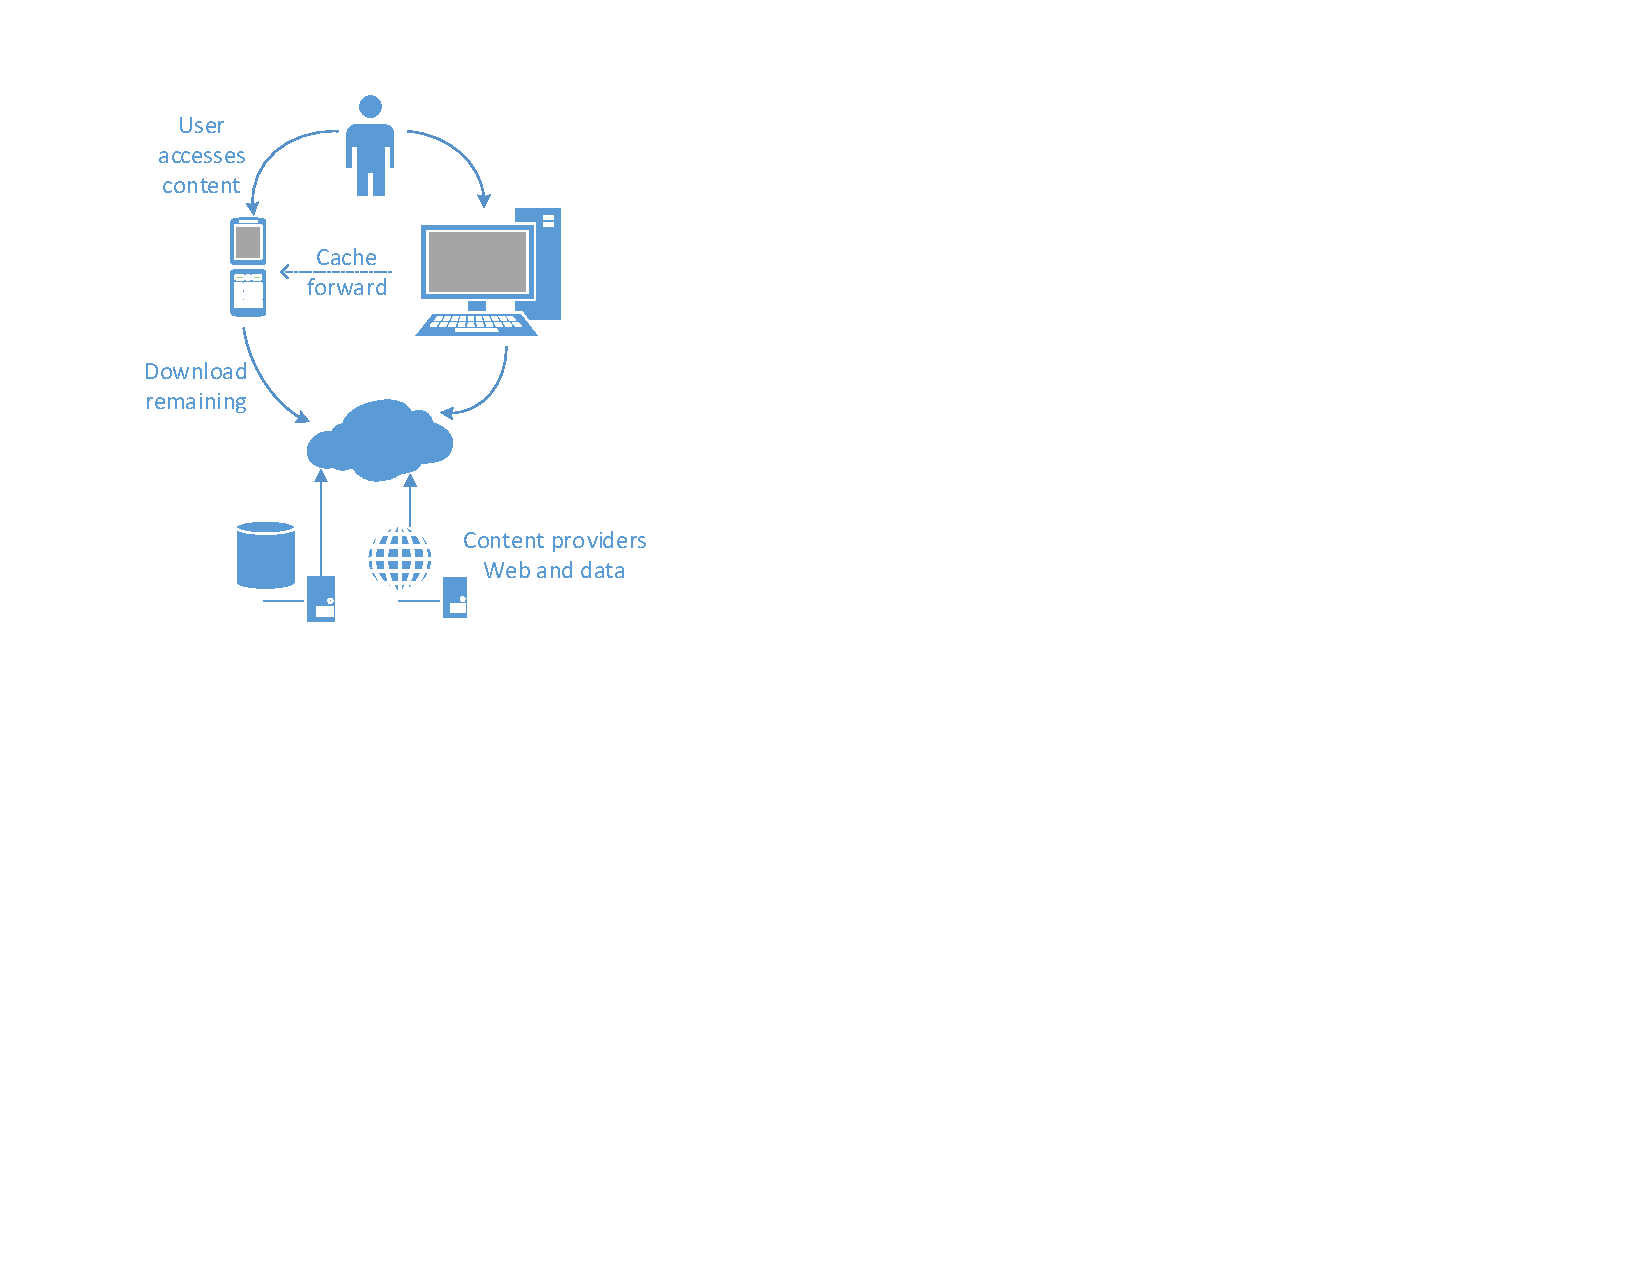
\includegraphics[width=.925\linewidth]{Drawing1}
	\caption{Overall setup of world wide web based content access by a user over time using primary and secondary devices to display the same content. If the devices are able to synchronize their caches through short-range communications, energy savings become possible.}
	\label{fig:setup}
\end{figure}
As most devices are charged over night, or are at least stationary within local area network ranges, we propose to utilize this general idle period to allow direct forwarding of cached objects.
We presume that browser clients will have a shared information source in the cloud that allows the identification of visited web pages, an approach most browser clients take to date.
In turn, clients are enabled to identify web page objects that are identical between the different device display modalities, i.e., identical web objects delivered when requesting a desktop/mobile versions of a web page.
The thus transmitted objects, in turn, reside locally within the mobile device cache and do not require an energy--expensive mobile download through cellular interfaces. 
We note that the reverse of this approach is possible as well.
To support our approach, we gather data through the publicly accessible \url{WebpageSpeedTest.org} website as well as the \url{httparchive.org} archive of a large dataset of performance evaluations for popular web pages; we refer the interested reader to~\cite{Me13} for a more detailed discussion.

The remainder of this paper is structured as follows.
In the following section, %we describe our overall scenario before 
we provide an example based on a particular news web page.
In the subsequent Section~\ref{s:large}, we discuss the overall properties of a large web page dataset archive and provide a description for the simulation-driven evaluation of our approach. 
We discuss the obtained results in Section~\ref{s:results} before concluding in Section~\ref{s:conc}.


%\section{Scenario Description }





\section{Individual Example}
\label{s:example}
In this section, we outline an individual example for the German news web page ``Der Spiegel,'' accessible at \url{http://www.spiegel.de}.
This web page serves as an example for a rich media and advertising material containing web presence that is frequently updated.
On February 12, 2014, we performed a speed test online using ($i$) Internet Explorer 9 as the browser instance for a desktop client, ($ii$) Chrome as the mobile browser on a Google Nexus 5 instance, and ($iii$) Safari for an iPhone 4 instance provided by \url{WebpageSpeedTest.org} (both mobile clients were traffic shaped to 3G connection emulations).
An example screenshot of the web page as rendered is provided in Figure~\ref{fig:screens}.
\begin{figure}
	\centering
	
\includegraphics[width=.95\linewidth]{1screen}
	\caption{Screenshot of rendered web page from WebPageSpeedTest.org. As illustrated, the main textual and pictorial content items are flanked by background and interactive advertisements.}
	\label{fig:screens}
\end{figure}
As illustrated, the web page exhibits a significant amount of objects that are required for advertisements, visual items (images, layout), and scripting.
%\subsection{Metrics}
We evaluate the reported data as follows. 
For each display modality and browser client, we gather the individual web objects requested and the response sizes and headers for caching information (for HTTP response codes 200 only, as we are not interested in redirects).
We denote the number of all objects returned for a request modality (i.e., Internet Explorer for the desktop client example and iPhone or Nexus 5 for mobile counterparts) as $N$, their average size as $\overline{X}$, the standard deviation of their sizes as ${\sigma}_{X}$, and the Coefficient of Variation (CoV) of the returned object sizes as $\mathrm{CoV}_{X}$. 
As in the HTTP specification, the \emph{max--age} directive overrides others, so we initially consider that directive for the cache longevity of the individual objects. 
If no explicit information is found, we consider the response header's \emph{expires} information, which provides a secondary cache lifetime. 
If both are not found, or if the \emph{expires} date is in the past or right at the request time, we set the cache lifetime to zero. 
Similar to the notation for the object sizes, we denote the expiration time characteristics as $\overline{T}$, $\sigma_{T}$, and $\mathrm{CoV}_{T}$, respectively.
%In case of size differences between the three, we utilize the smallest size as lower boundary.


\subsection{Data Description}

We provide an initial high-level overview of the web page characteristics for \url{http://www.spiegel.de} as requested by the different clients in Table~\ref{tab:spiegel}.
\begin{table}
\centering
\caption{High-level overview of different client web page statistics for http://www.spiegel.de}
\label{tab:spiegel}
\begin{tabular}{|l|r|r|r|}
	\hline
	Statistic          & IE Deskt. &    iPhone &   Nexus 5 \\ \hline
	$N$                &       154 &       132 &       145 \\ \hline\hline
	$\overline{X}$     &  10402.77 &   8846.39 &  10201.63 \\ \hline
	$\sigma$           &  19103.19 &  13438.05 &  25684.58 \\ \hline
	$\mathrm{CoV}_{X}$ &      1.84 &      1.52 &      2.52 \\ \hline\hline
	$\overline{T}$     & 106285.14 & 114780.69 & 114818.28 \\ \hline
	$\sigma_{T}$       & 125080.27 & 125576.65 & 126090.90 \\ \hline
	$\mathrm{CoV}_{T}$ &      1.18 &      1.09 &      1.10 \\ \hline
\end{tabular}
\end{table}

We initially observe that the desktop version (with Internet Explorer 9 as requesting browser client) exhibits the highest number of objects, followed by the mobile Chrome/Android and Safari mobile/iOS versions.
Interestingly, there is only a minor difference in the number of objects between these versions.
Next, we observe that the trend for the average number of bytes is aligned with the number of elements. 
In total, the mobile Chrome version is almost on par with the desktop one (at 92~\% of total data); only the Safari mobile version seems optimized (at 72~\% of total data).
The standard deviation and Coefficient of Variation (CoV) amongst individual element sizes are highest for the mobile Chrome version, indicating more significant size differences than for the safari version (which is one unit lower), while the desktop version falls into the middle.

Next, we evaluate the elements' caching properties on a high level as presented in Table~\ref{tab:spiegel} as well. 
Overall, we note that the highest average caching time is observed for the mobile Chrome access with the Nexus 5 device, trailed immediately by the iOS access and (with distance) by the desktop browser.
We note that the overall variability in terms of expiration times amongst elements is fairly low and comparable, as indicated by CoV values around 1.1.

\subsection{Evaluation of Local Cache Forwarding}
We now shift the view to the possibility for identical objects to be re--utilized locally to avoid additional download penalties in time and energy consumption.
Simultaneous with a web page request, a local broadcast could ``ask'' for the cached elements for a website to be delivered locally from participating clients. 
Alternatively, cellular provisioning methods, such as in LTE--A, could initiate the device--to--device local exchange as well.
Once the request is received, the local coordination can take place, which inherently results in the forwarding of elements that are the same across browser instances and which have a future cache lifetime expiration.

We filter out elements that are not similar amongst the different requesting devices, which results in 82 objects with the same URL and size combination. 
In other words, just above half of the objects constituting the web page under consideration are identical between different clients.

While we note an identical cache lifetime for most of these objects, a slight increase is notable from the Desktop over Safari to Chrome clients.  
Next, we remove items that exhibit a cache lifetime of zero for any of the three requesting clients, resulting in 59 objects.
These remaining objects display a reduced average cache lifetime for the mobile browsers, whereby mobile Chrome exhibits the shortest.
In turn, we choose the iOS Safari mobile as our exemplary base for calculations. 
We utilize the approximations for energy consumptions presented in~\cite{PeFiWi11} to determine the amount of energy required if local data forwarding can be performed using either Bluetooth or WLAN technologies. 
We illustrate the energy consumption as function of time in Figure~\ref{fig:ios_time_energy}.
\begin{figure}
	\centering
	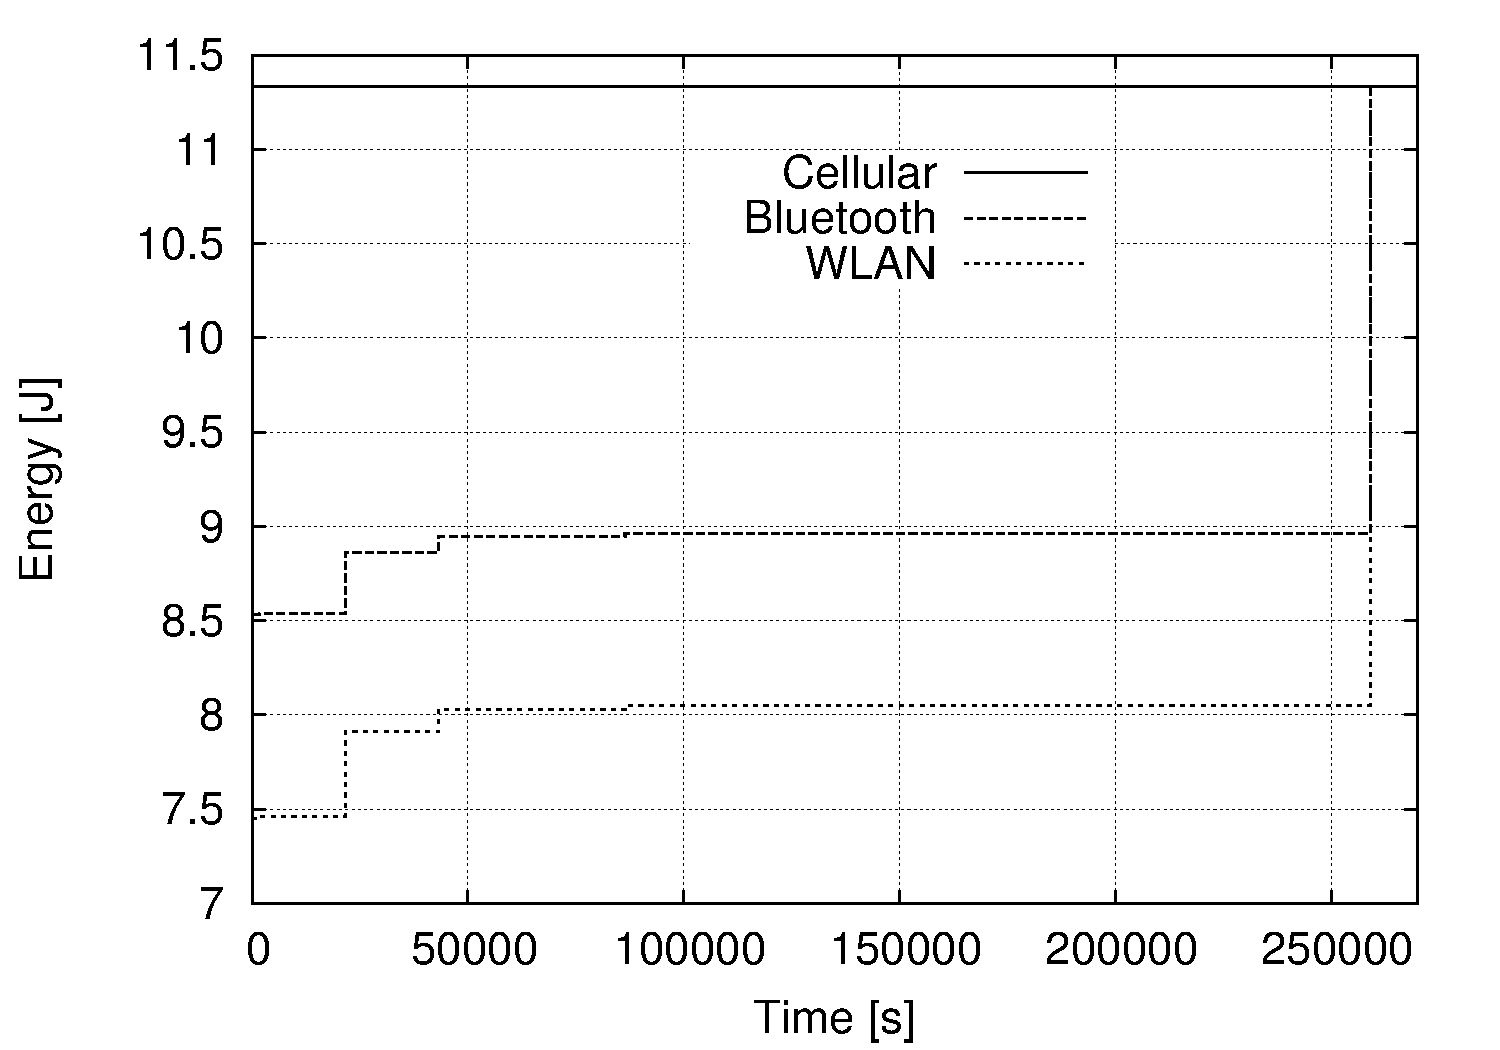
\includegraphics[width=\linewidth]{energy_ios_time}
	\caption{Energy required to download web page data via cellular connection or through combination with partial local exchange with Bluetooth/WLAN.}
	\label{fig:ios_time_energy}
\end{figure}
The complete download energy for exclusive use of cellular is the upper limit on energy spent downloading the data associated with the web page. 
The Bluetooth and WLAN data exchanges with other local clients both follow the same underlying trend with increasing energy required to transmit all data as time progresses from the last access point in time (due to cache expirations).

We illustrate the relative amount of data/items within the cache in addition to the attainable savings in Figure~\ref{fig:rel_ios_time} as a function of delayed access time. 
\begin{figure}
	\centering
	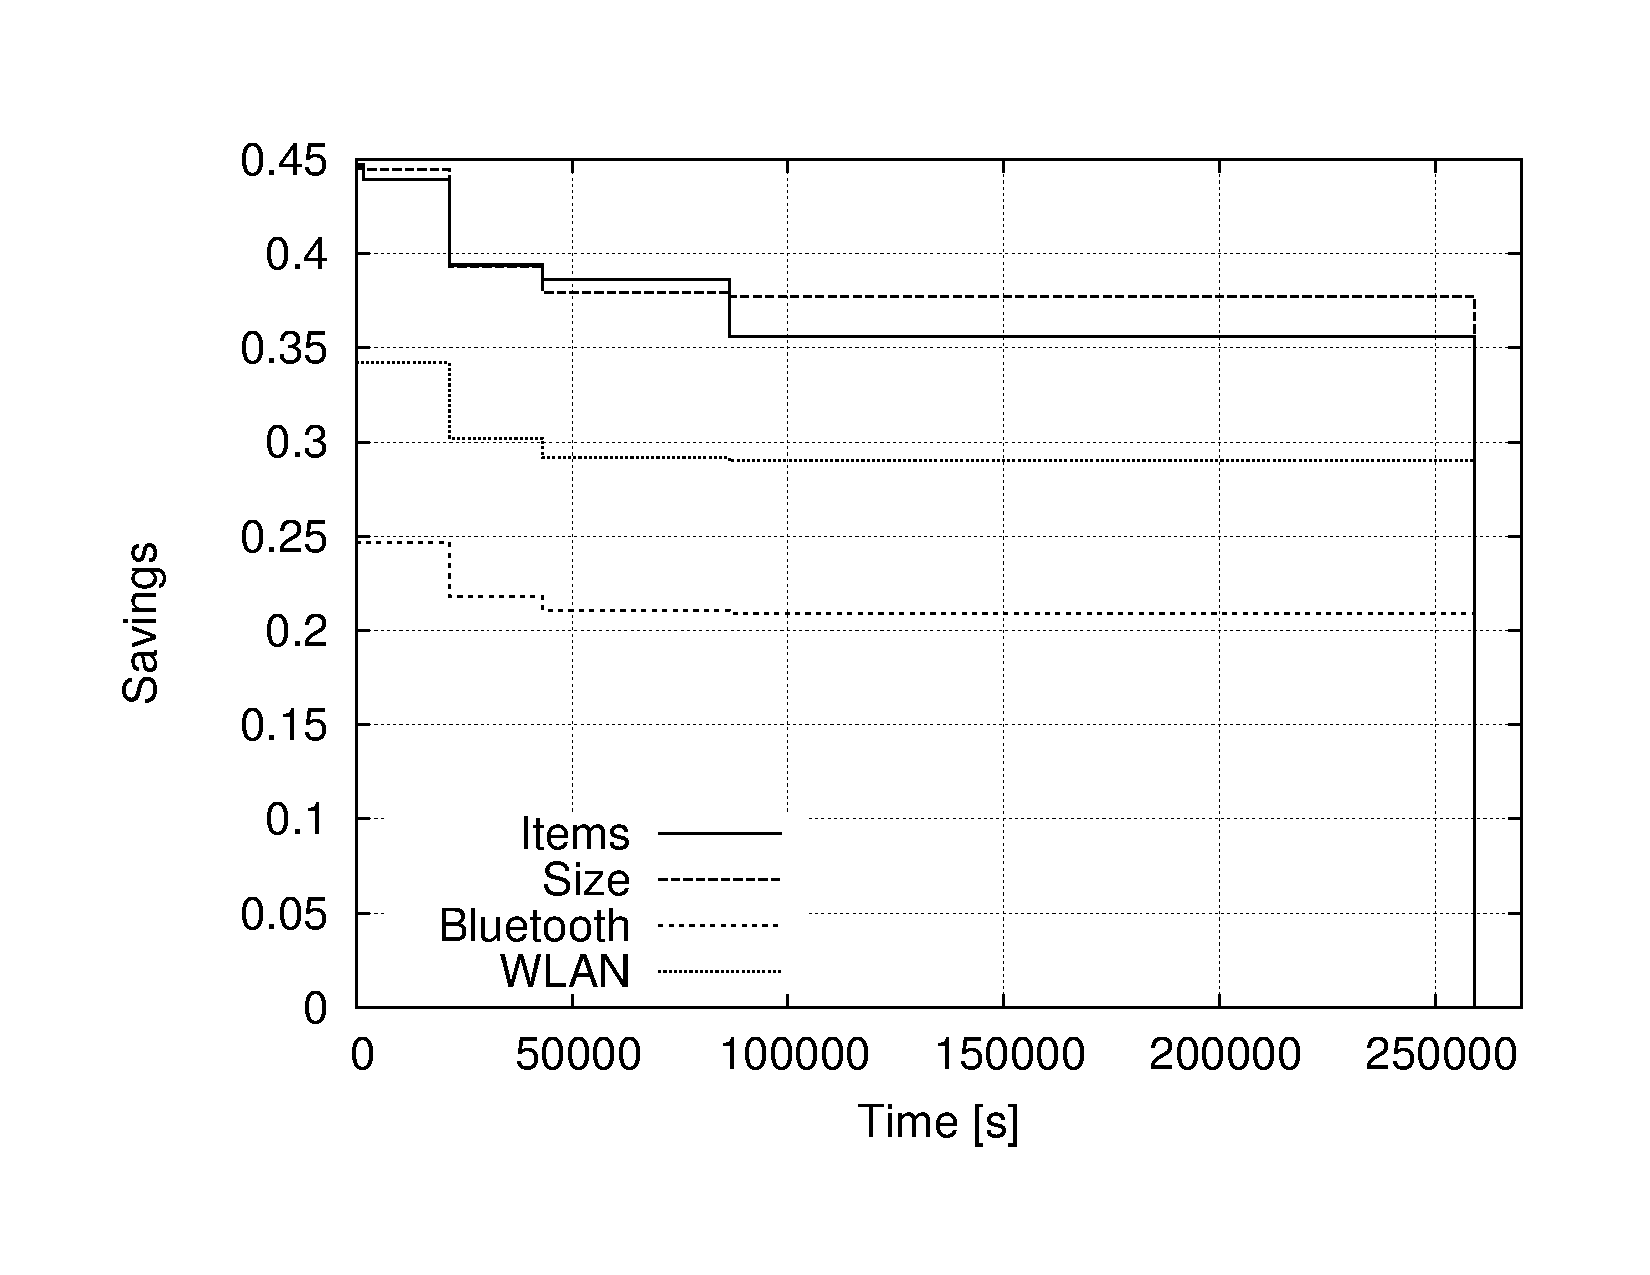
\includegraphics[width=\linewidth]{rel_ios_time}
	\caption{Relative number of items and data amounts in cache and savings resulting from local data exchange with a desktop client.}
	\label{fig:rel_ios_time}
\end{figure}
We observe that a significant amount of the overall data can be cached (and would in turn be suitable for localized forwarding).
We additionally observe that even for longer durations up to multiple days, significant amounts of data remain in the cache.
Combining the forwarding from locally cooperating clients, e.g., user-owned desktop computer in the same network through either Bluetooth or WLAN technologies, we utilize the approximations outlined in~\cite{Se13} to derive the relative gains of our approach in terms of energy consumption. 
Specifically, we compare our approach (combining locally forwarded cached objects and cellular downloads of the remainder) with the regular download of all objects through the cellular network interface. 
We note that significant savings above 20 \% are attainable with our approach, even if the filling of the device's cache is performed wirelessly as well.



\section{Large Dataset Performance Evaluation}
\label{s:large}
We now evaluate our proposed approach through simulations based on a large dataset of landing web pages of popular websites.
For this purpose, we retrieved the publicly available web page response details from \emph{httparchive.org} and created a subsequent dataset for October 1st, 2013.

\subsection{Dataset Description}
The dataset we utilize for the performance evaluation contains the individual web responses for the most popular websites of fixed (Internet Explorer for the desktop) and mobile (iOS for iPhone 4) websites, ranked through the Alexa popularity index.
Furthermore, the dataset contains the individual response details, including cache expiration times and sizes. 

Similar to the individual web page example, we provide an overall description of the response sizes and maximum expiration ages in Table~\ref{tab:dataset}.
\begin{table*}
\centering
\caption{Overview of the large dataset characteristics for all pages and response objects with a focus on the cache lifetime.}
\label{tab:dataset}
\begin{tabular}{|l||c|c|c|c||c|c|c|c|}
	\hline
	Category                         & \multicolumn{4}{|c||}{Desktop (IE)}                       & \multicolumn{4}{|c|}{Mobile (iOS)}                      \\
	                                 & $\sum X_i $ &   $N$    & $\sigma(X_i)$ & $\overline{X_i}$ & $\sum X_i $ &  $N$   & $\sigma(X_i)$ & $\overline{X_i}$ \\
	                                 &    [MB]     &          &     [kB]      &       [kB]       &    [MB]     &        &     [kB]      &       [kB]       \\ \hline\hline
	expAge $<$ 30 Seconds            &  238490.28  & 15670679 &    1698.59    &      15.22       &   1355.24   & 122598 &    582.98     &      11.05       \\ \hline
	30 $\le$ expAge $<$ 1 Minute     &   170.94    &  29130   &     27.38     &       5.87       &    12.68    &  898   &     70.38     &      14.12       \\ \hline
	1 Minute $\le$ expAge $<$ 1 Hour &  15192.40   &  797450  &    270.06     &      19.05       &   282.36    & 15854  &    226.62     &      17.81       \\ \hline
	1 Hour $\le$ expAge $<$ 12 hours &  29798.68   & 1186947  &    751.45     &      25.11       &   244.14    & 17424  &    209.84     &      14.01       \\ \hline
	12 hours $\le$ expAge $<$ 1 day  &   6188.57   &  358998  &    227.63     &      17.24       &    91.37    &  5952  &     91.37     &      15.35       \\ \hline
	1 day $\le$ expAge               &  195784.64  & 9888147  &    1337.36    &      19.80       &   2122.96   & 126629 &    750.51     &      16.77       \\ \hline\hline
	Average                          &  80937.59   & 4655225  &    718.75     &      17.39       &   684.79    & 48226  &    321.95     &      14.20       \\ \hline
\end{tabular}
\end{table*}
We note that the overall average response size as result of desktop requests (when batched into the outlined time frames) is around 17 kB, with the largest average sizes occurring between one and twelve hours.
Mostly, we note that the majority of objects exhibit a short expiration time between zero and 30 seconds.
For the responses to mobile devices, we note that the majority of objects are in the same short time span and the long time span of more than one day.
The highest average response sizes, however, are observed between one hour and half a day, in difference to the desktop counterpart.
For more details of the differences between fixed and mobile web pages, we refer to~\cite{JoSe14Commag}.

We illustrate the cumulative distribution for the desktop and mobile client response expiration ages in Figure~\ref{fig:comp_cpd}.
\begin{figure}
	\centering
	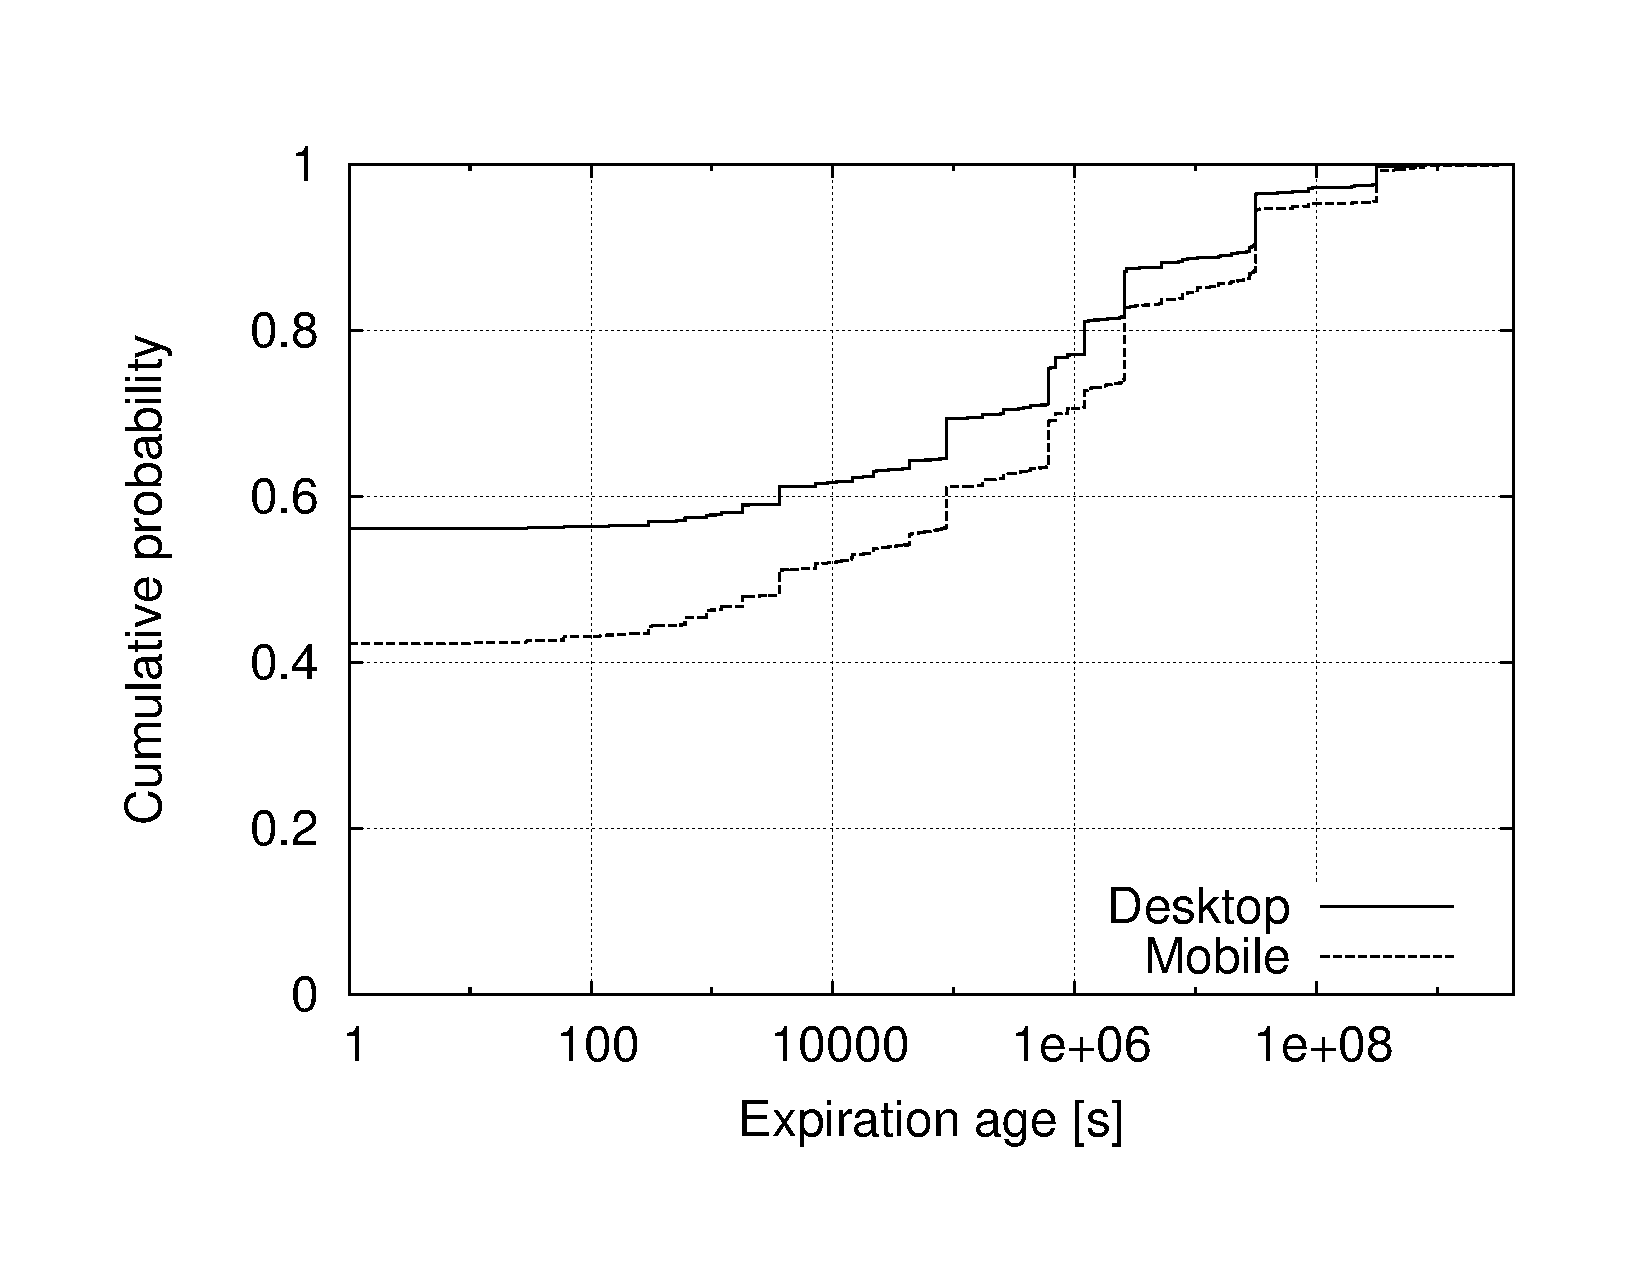
\includegraphics[width=\linewidth]{comp_cpd}
	\caption{Cumulative probability of expiration times for desktop and mobile responses.}
	\label{fig:comp_cpd}
\end{figure}
We observe that a significant portion ($>40$ \%) of responses from web servers exhibits an immediate expiration and would, in turn, require an immediate retrieval by clients.
The cumulative expiration probability is higher for responses to desktop clients, which can be attributed to the typically more abundant bandwidth (and less optimization requirements) in contrast to a mobile setting (where web content developers might be more considerate of limitations).
In addition, we perform matching of request to mirror the individual example with a direction from desktop to mobile client. 


\subsection{Simulation Model Description}
%\ref{we use the simple zipf distribution to make life easy?} 
We evaluate the effectiveness of our approach through simulation, which we perform as follows.
For the time period of one week, we randomly select a web page from the mobile dataset and separate the data that is required to be downloaded and the data that is still available in cache due to the maximum expiration age of the individual objects. 
We subsequently wait for a random amount of time before repeating the procedure.
%We now describe the process in greater detail.


Initially, we sort all landing web pages $l, l=0,\ldots,L$ from the 
%Oct. 1 dataset in the \emph{httparchive.org} 
dataset based on their popularity ranking.
To simulate the popularity of web pages, it was found that the Zipf distribution effectively describes the popularity of individual requests. %, see, e.g., \cite{}. 
%While an augmented Zipf-like distribution, which enhances the ``traditional'' Zipf distribution to adjust for non-compensated effects, was presented in \cite{KrTeSh06}.
We chose to utilize the non-modified Zipf distribution for our simulation purposes, noting that additional modifications to the distribution exist that can further enhance it, see, e.g., \cite{KrTeSh06}.
For the total number of web pages $L$, we derive the probability of page $l$ being selected in turn as
\begin{equation}
p(l)=\frac{l^{-\alpha}}{\zeta(l)},
\end{equation}
where $\zeta(\cdot)$ denotes the Zeta function. 
We furthermore set $\alpha=0.85$ as an average choice in common ranges utilized for this parameter.
%Specifically, the authors introduced $f_r = a + \frac{b}{(c+r)^\alpha}$, whereby $r$ denotes the rank under consideration. 
%Through evaluation of different web proxy server caches, the authors found that approximations for the variables were comparable; in turn, we utilize the described values of $a=-7.62\cdot 10^{-6}$, $c=5.05$, and $\alpha=1.03$, which the authors found for a broad range of sites in their evaluation. 
%% Lastly, $b$ is calculated as $b=\frac{1}{\sum_{n=1}^{N}\frac{1}{n^{\alpha}}}$.
%% We determine $b \approx 5.6305$.
%% for N=5000 it's 8.095576472991269


Once the individual mobile web page $l$ was randomly chosen, we compare it to its desktop counterpart, with $\left\{ d,m \right\}$ denoting the request modality.
As each page $l$ exhibits a time-sensitive number of responses, we denote them as $r^{\left\{ d,m \right\}}(l,t)$ and each page exhibits $R^{\left\{ d,m \right\}}(l,t=0)$ in total.
Let $t_c(r^{\left\{ d,m \right\}}(l))$ denote the expiration or max-age directive received with the response at $r^{\left\{ d,m \right\}}(l,t=0)$.
The number of objects or responses to be retrieved at time $t$ in turn are given as 
\begin{equation}
R^{\left\{ d,m \right\}}(l,t) = \sum_{r^{\left\{ d,m \right\}}(l,0)} \left[ t_c(r^{\left\{ d,m \right\}}(l)) \ge t \right]
\end{equation}
where $\left[ \cdot \right] $ denotes the Iverson Bracket.
In the following, we abbreviate to $t_c$ for readability when in direct context.

We furthermore denote the size of the individual response retrieved at time $t$ as 
\begin{equation}
x_{r}^{\left\{ d,m \right\}}(l,t) = x_{r}^{\left\{ d,m \right\}}(l,0) \cdot \left[ t_c \ge t \right].
\end{equation}
The total size of objects or responses retrieved at simulation time $t$ thus is given as 
\begin{equation}
X^{\left\{ d,m \right\}}(l,t) =\sum_{r^{\left\{ d,m \right\}}(l,0)} x_{r}^{\left\{ d,m \right\}}(l,t).
\end{equation}


For performance evaluation purposes, we simulate the user behavior similar to the process outlined in~\cite{AnCoGrPa03}, whereby we randomly draw the time between requests $t_u$ as Pareto distributed using
\begin{equation}
p(t_u)=\beta k^\beta t_u^{-(\beta+1)},
\end{equation}
 with $\beta=1.5$, $k=30$.
We assume that no delays are accrued due to instantaneous cache retrievals or downloads. 
Using time index $i$, we thus derive $t_{i+1}=t_i + t_u$.
We continue the simulation until $t_{i+1} = t \ge T =  604800$ [s], i.e., one week.
To maintain tractability, we bundle the presented results into bins of 3600 seconds, i.e., one hour, through averaging.


%
%Simulation approach:
%sort pages by rank, assume this is the distribution
%map distribution zipf to webpage rank
%random draw time to wait (startup phase required?)
%random draw for zipf mapping of websites->draw prob, get rank
%
%
%Simulation
%1)Row Selected from spreadsheet (1->N, N= number of rows in spreadsheet, row number selected based on zipf distribution with alpha = 0.85)
%2)Get shared requests information from row.  
%3) Get sum of requests and bytes for page requests that haven’t expired
%4)Write sums to files
%5) Time += Pareto Value (pareto shape = 1.5, shifted + 30)
%6)If time less than $END_TIME$, go to step 1.



\section{Performance Evaluation Results}
\label{s:results}
%Cache Simulation (.py)
%Spreadsheet contains data of mobile and fixed pages that shared identical urls
%-contains columns that shows the properties of identical requests that exist between fixed and mobile pages and properties of that request
%-spreadsheet sorted based on mobile page rank
We present our results for the individual responses or web objects and the total number of bytes.
We note that through approximations, such as the ones described in Section~\ref{s:example}, an inference of energy consumption would be possible as well.
We perform the simulations with an average $\alpha=0.85$ for the utilized Zipf distribution and repeat each week-long evaluation 2000 times.

\subsection{Web Page Objects and Bytes}
Initially, we present the total number of responses and bytes that would not require a download (i.e., would reside in the mobile cache) as a function of time in Figure~\ref{fig:sim1}.
\begin{figure}[h!]
	\centering
	\subfloat[Objects]{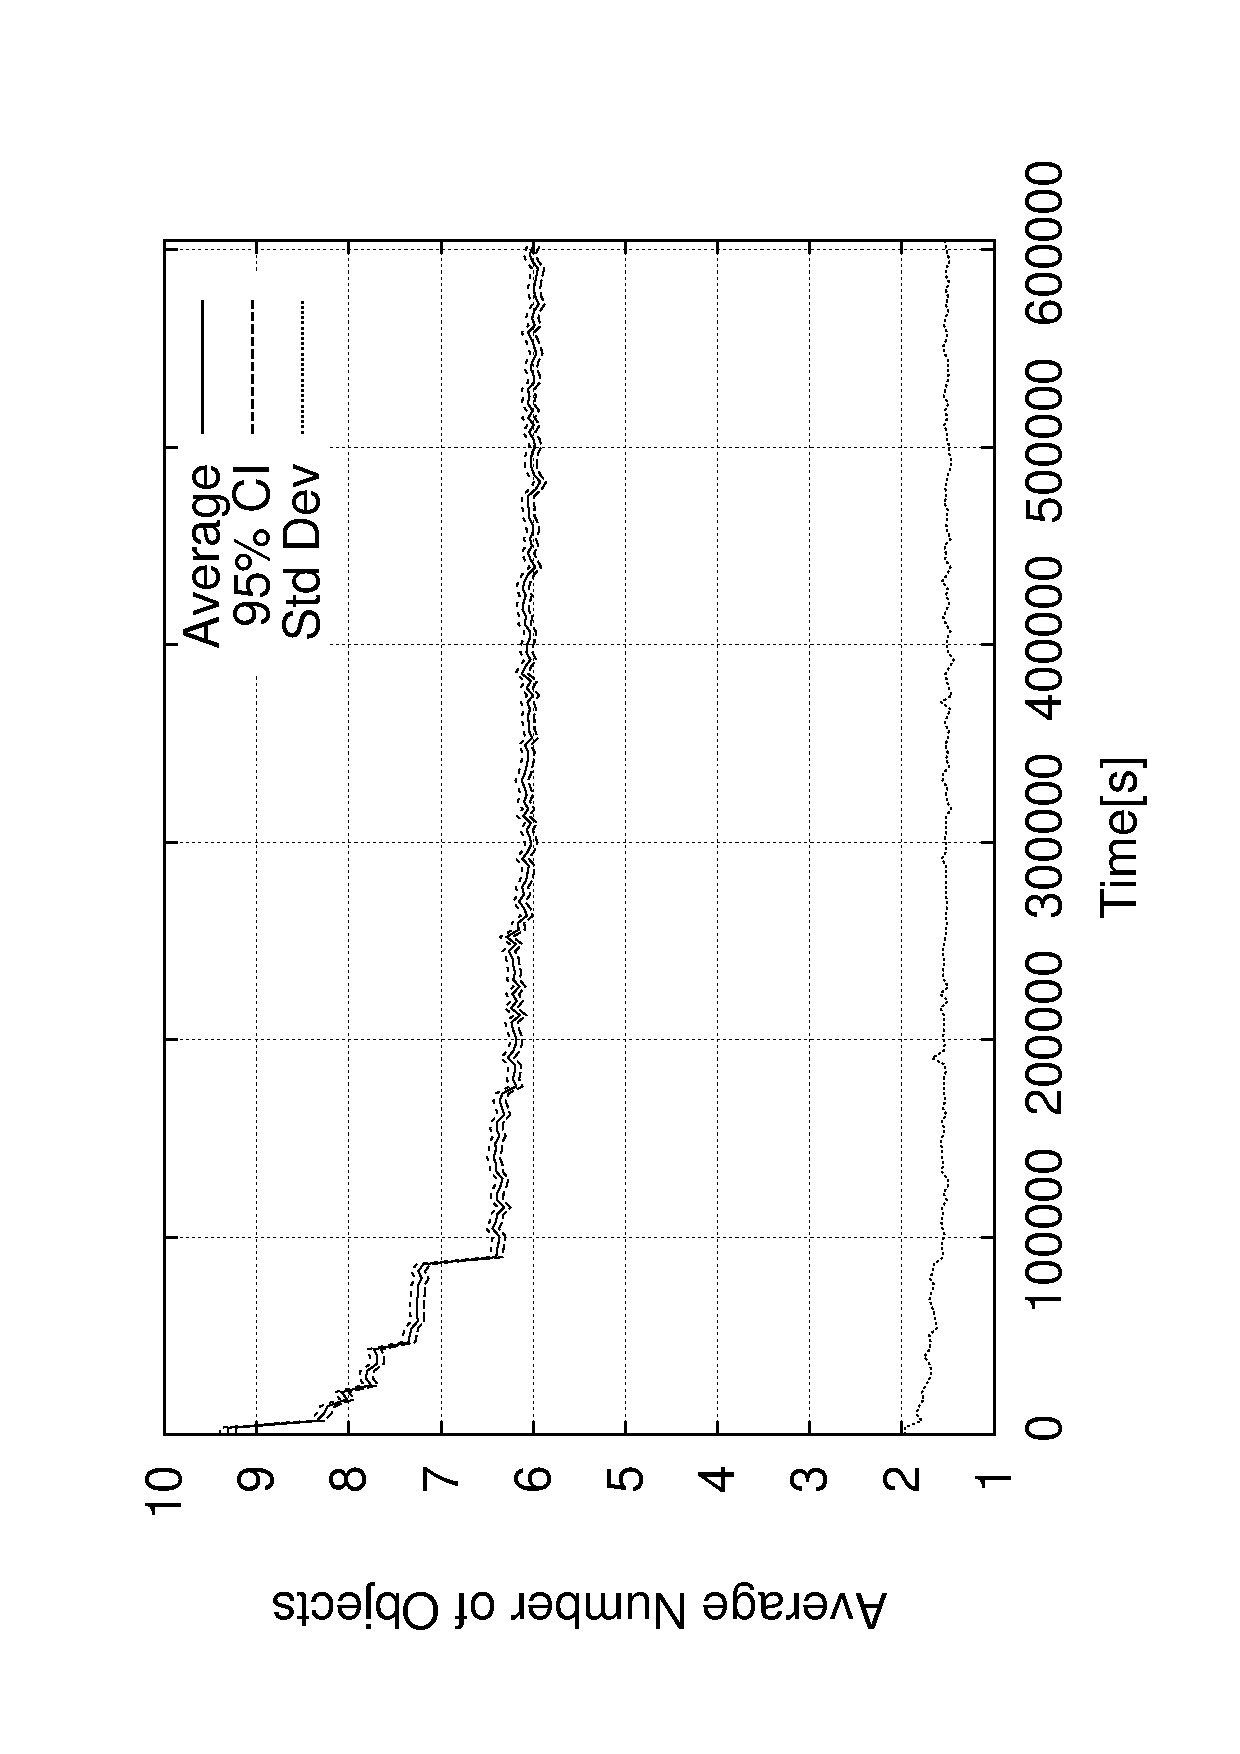
\includegraphics[width=.5\textwidth]{Fig6-a}
	\label{fig:simr_abs_reqs}}
	\qquad
	\subfloat[Bytes]{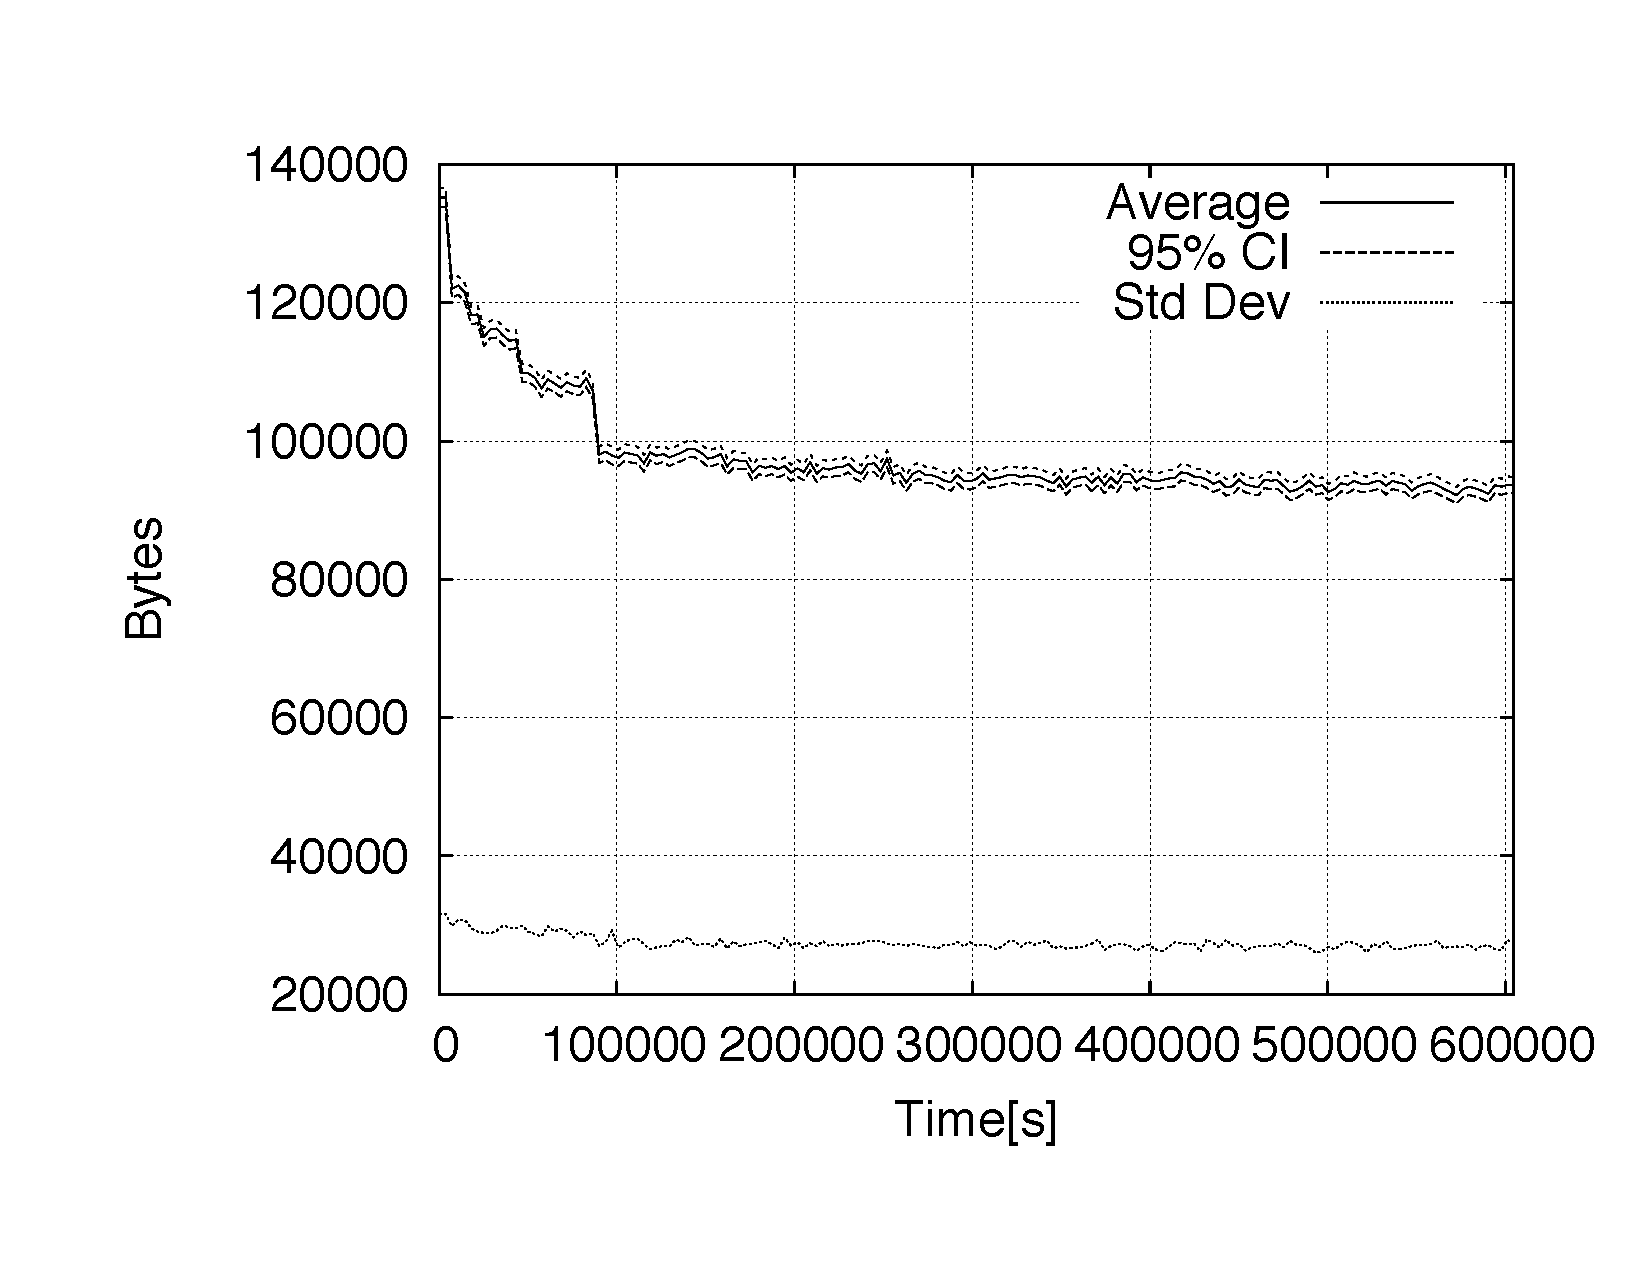
\includegraphics[width=.5\textwidth]{Fig6-b}
	\label{fig:simr_abs_byte}}
	\caption{Simulation results for the number of responses and bytes that are in the transfered mobile device cache as averages in 1-hour bins.}
	\label{fig:sim1}
\end{figure}

We note an immediate decrease in the number of requests, which is mirrored by the number of bytes as well (indicating a linear relationship as observed in, e.g., \cite{JoSe14Commag}).
We furthermore observe that the initial decline levels out at the simulation time of around one day, and  remains steady afterwards.
This indicates that within the simulation period of one week, initially a large number of items is non--shared between devices or exhibits no significant cache lifetime. 
In a following group of objects, cache lifetimes increase logarithmically, which leads to the exponential decline we observe here.
The narrow confidence intervals and low level of standard deviation indicate that the presented results are stable within simulation confines.
%\begin{figure}
%	\centering
%	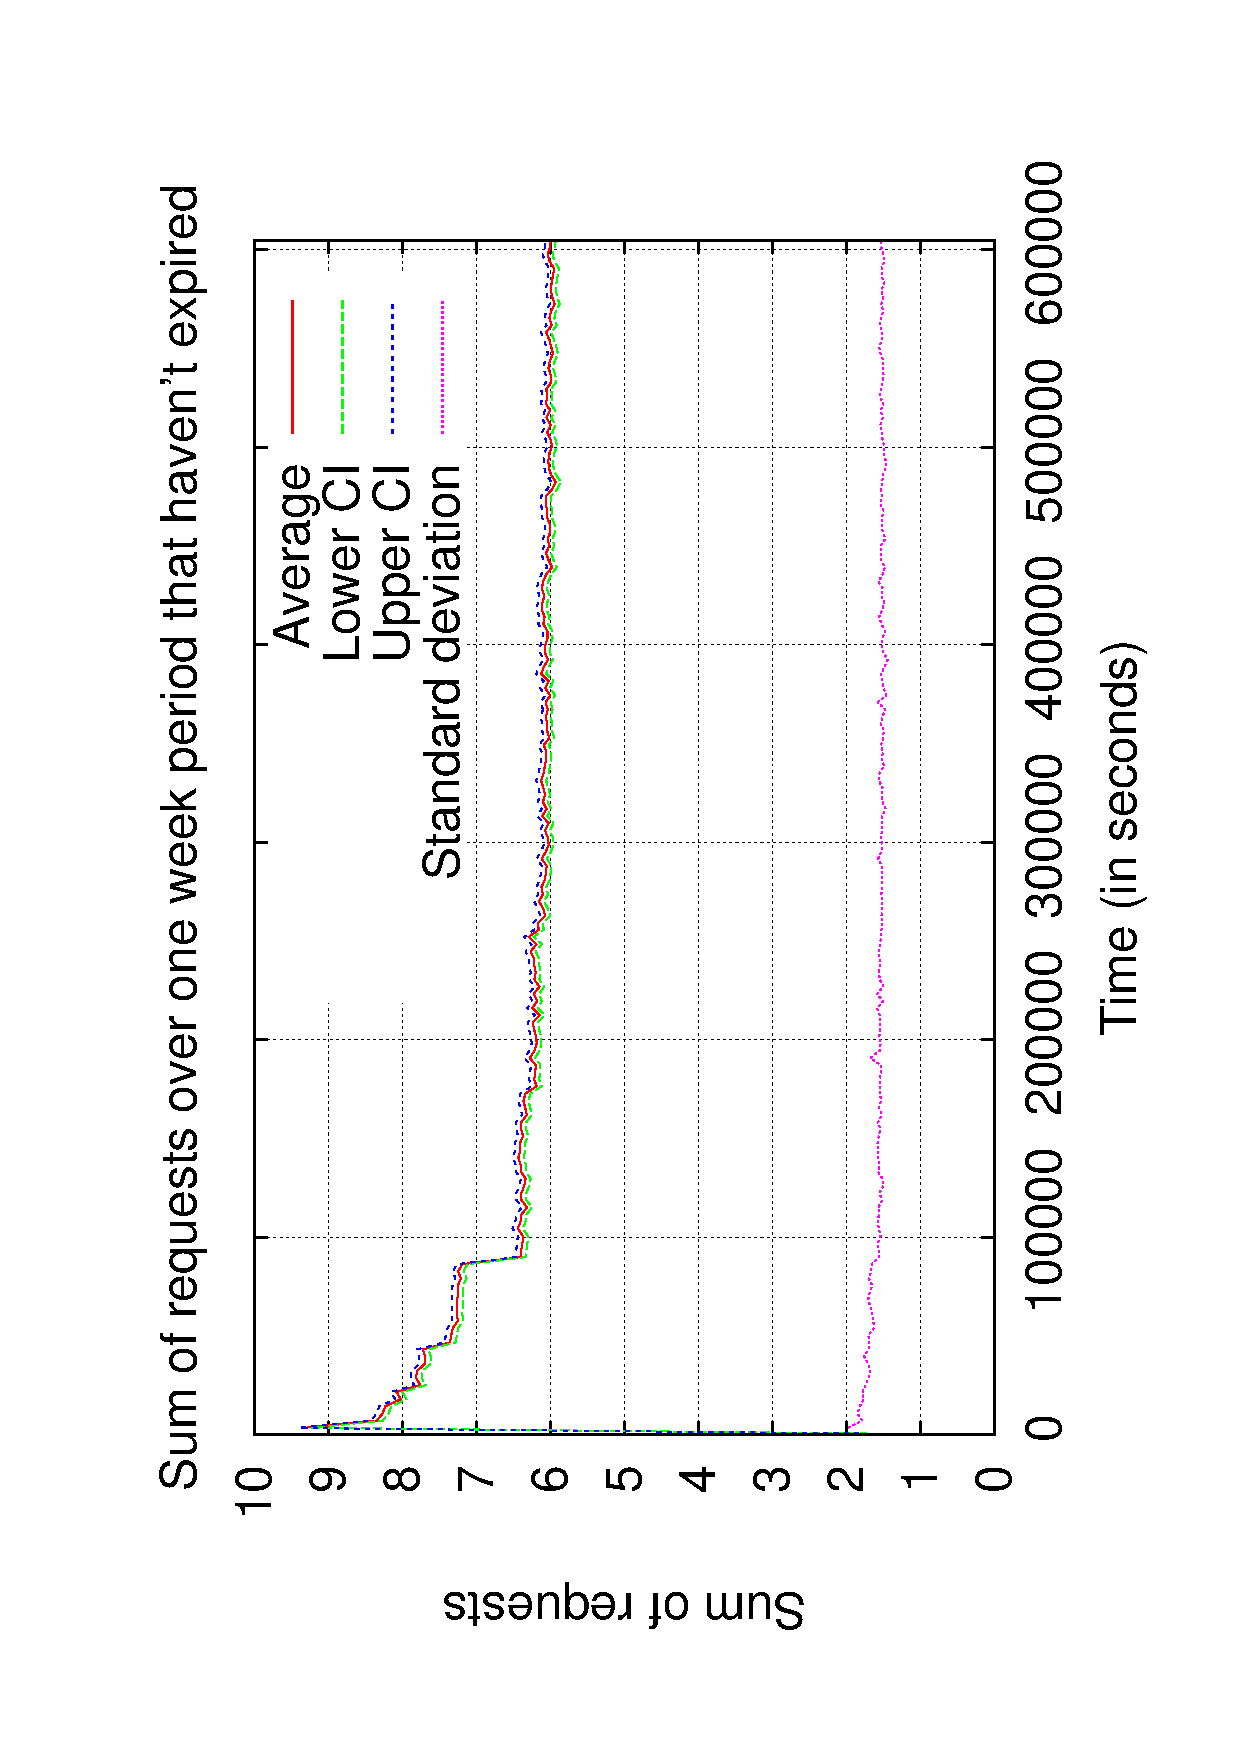
\includegraphics[width=.95\linewidth]{Sum_of_requests_over_time}
%	\caption{Sum of requests over time  }
%	\label{fig:sim_req}
%\end{figure}
%
%\begin{figure}
%	\centering
%	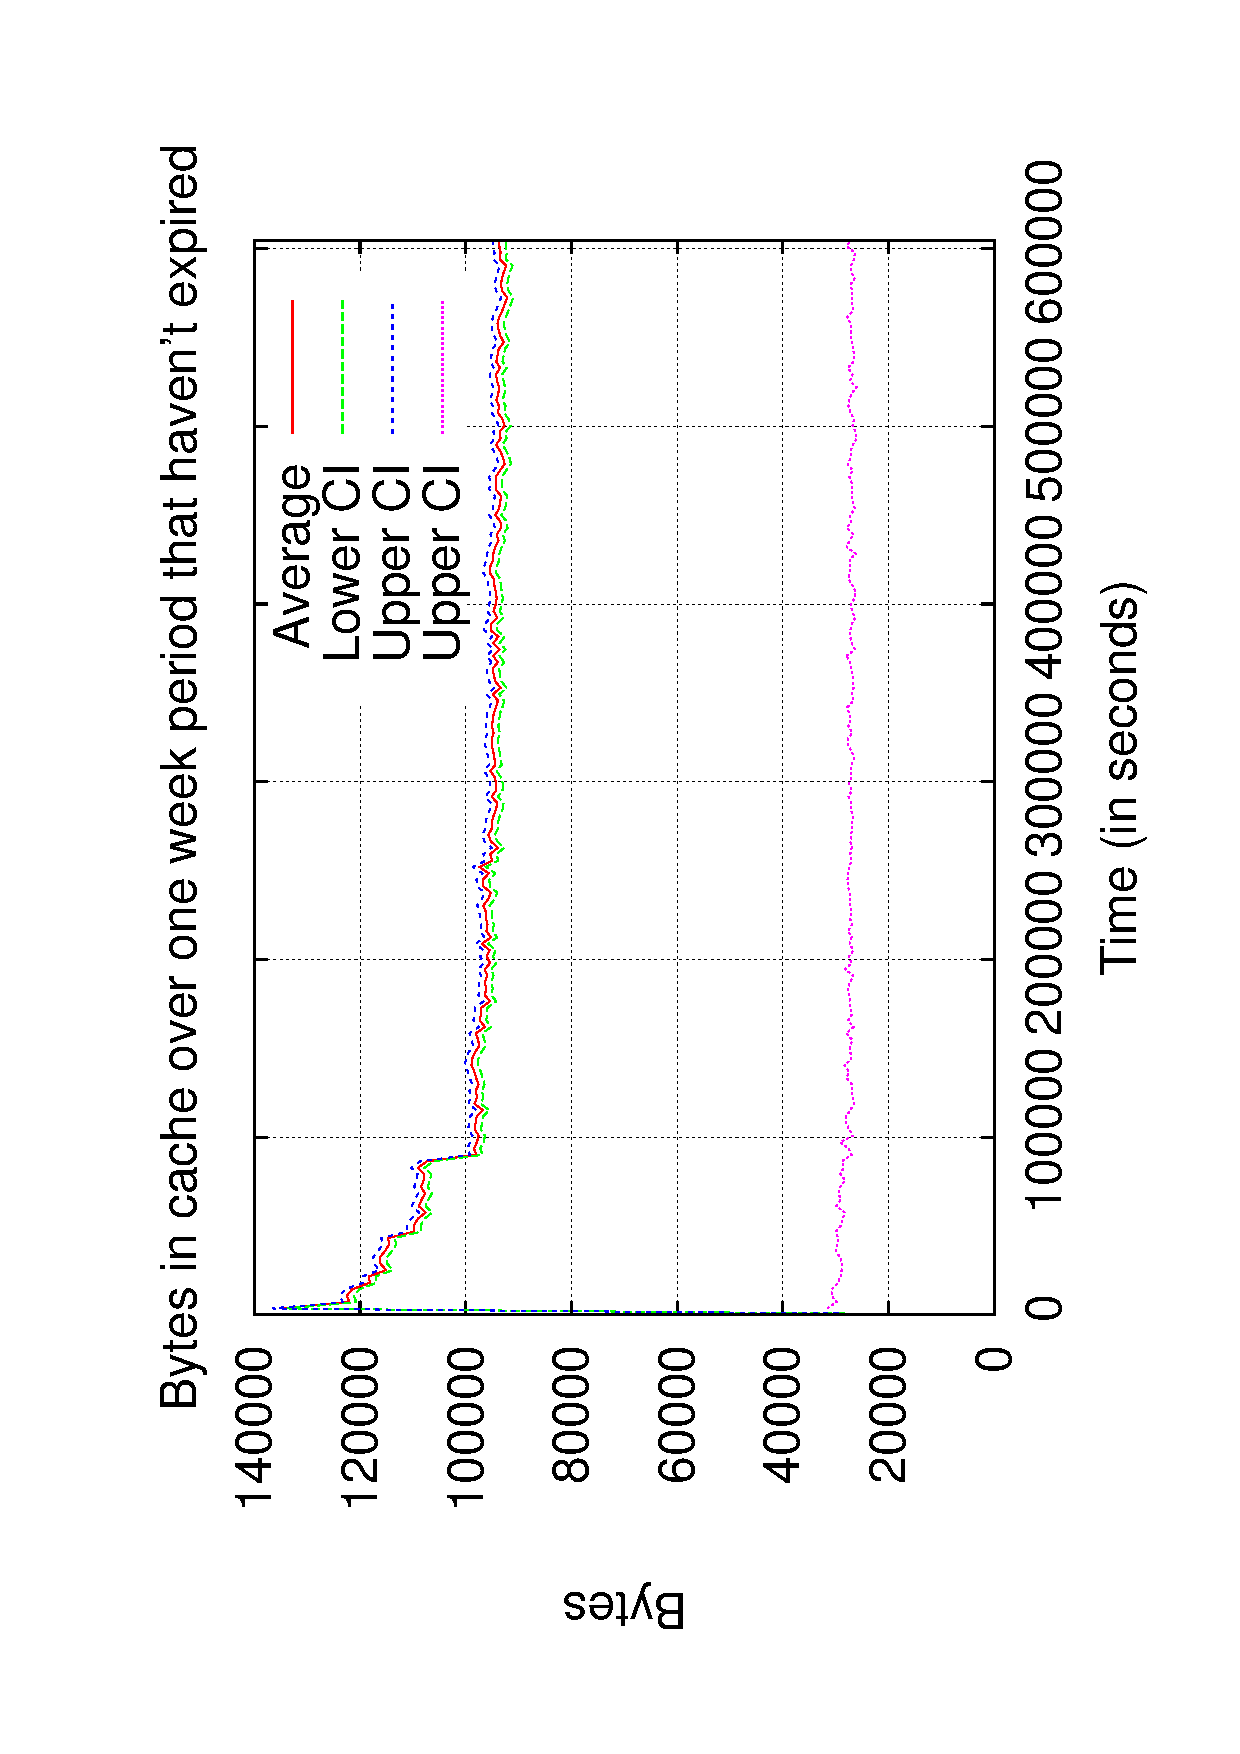
\includegraphics[width=.95\linewidth]{Sum_of_bytes_over_time}
%	\caption{Sum of requests over time  }
%	\label{fig:sim_bytes}
%\end{figure}

\subsection{Attainable Savings}
Next, we present how these findings translate into attainable savings with respect to requests for objects and bytes in Figure~\ref{fig:sim2} in relationship to the total web page data without caching.
\begin{figure}[]
	\centering
	\subfloat[Objects]{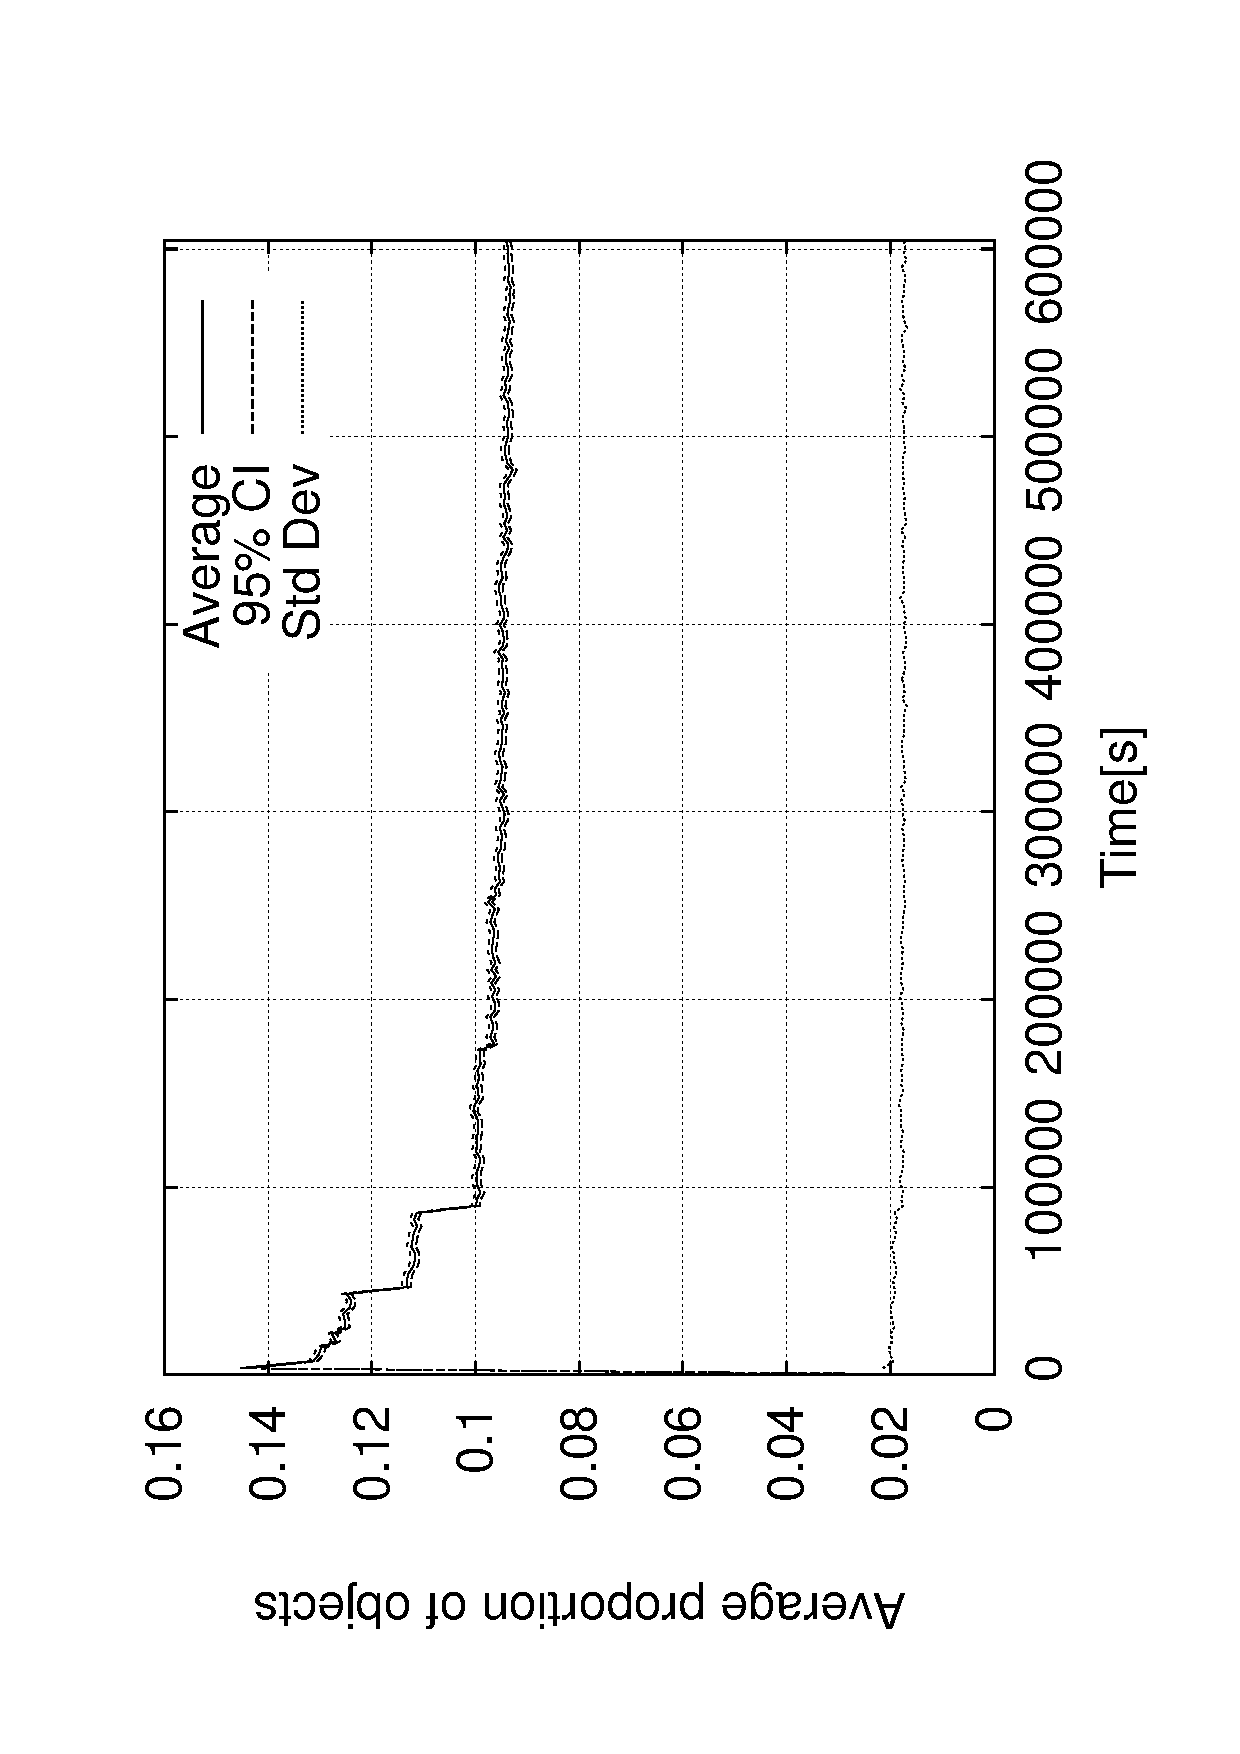
\includegraphics[width=.5\textwidth]{Fig7-a}
	\label{fig:simr_sav_reqs}}
	\qquad
	\subfloat[Bytes]{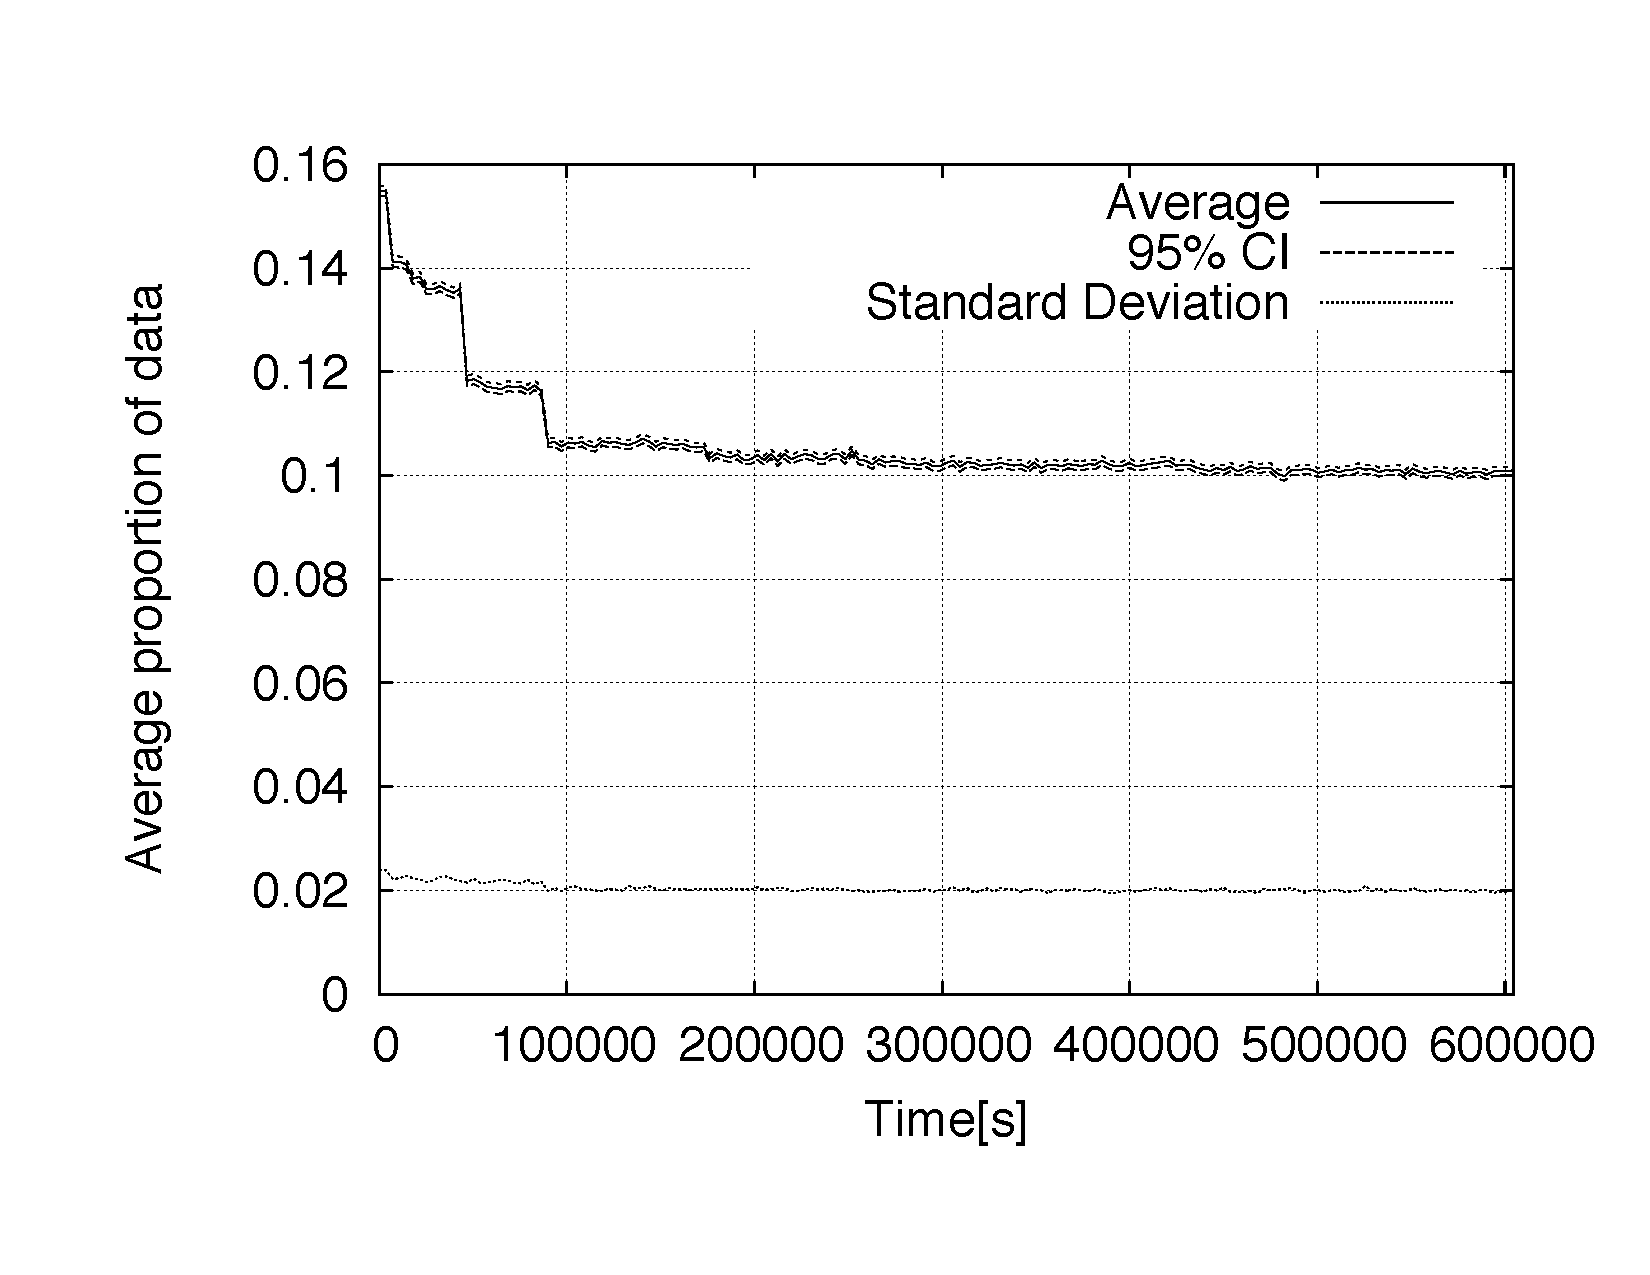
\includegraphics[width=.5\textwidth]{Fig7-b}
	\label{fig:simr_sav_byte}}
	\caption{Simulation results for the attained savings for the number of responses and bytes by transferring to the mobile device cache in 1-hour bins.}
	\label{fig:sim2}
\end{figure}
We initially note a declining trend similar to the one observed for the cached items in Figure~\ref{fig:sim1}, but with more distinct ``jumps'' observable at half-day and day times of the simulation.
Overall, we note that almost 15 \% savings for objects and bytes decline to around 10 \% after the boundaries of a day (whereby objects exhibit lower levels and bytes exhibit higher levels).


%\begin{figure}
%	\centering
%	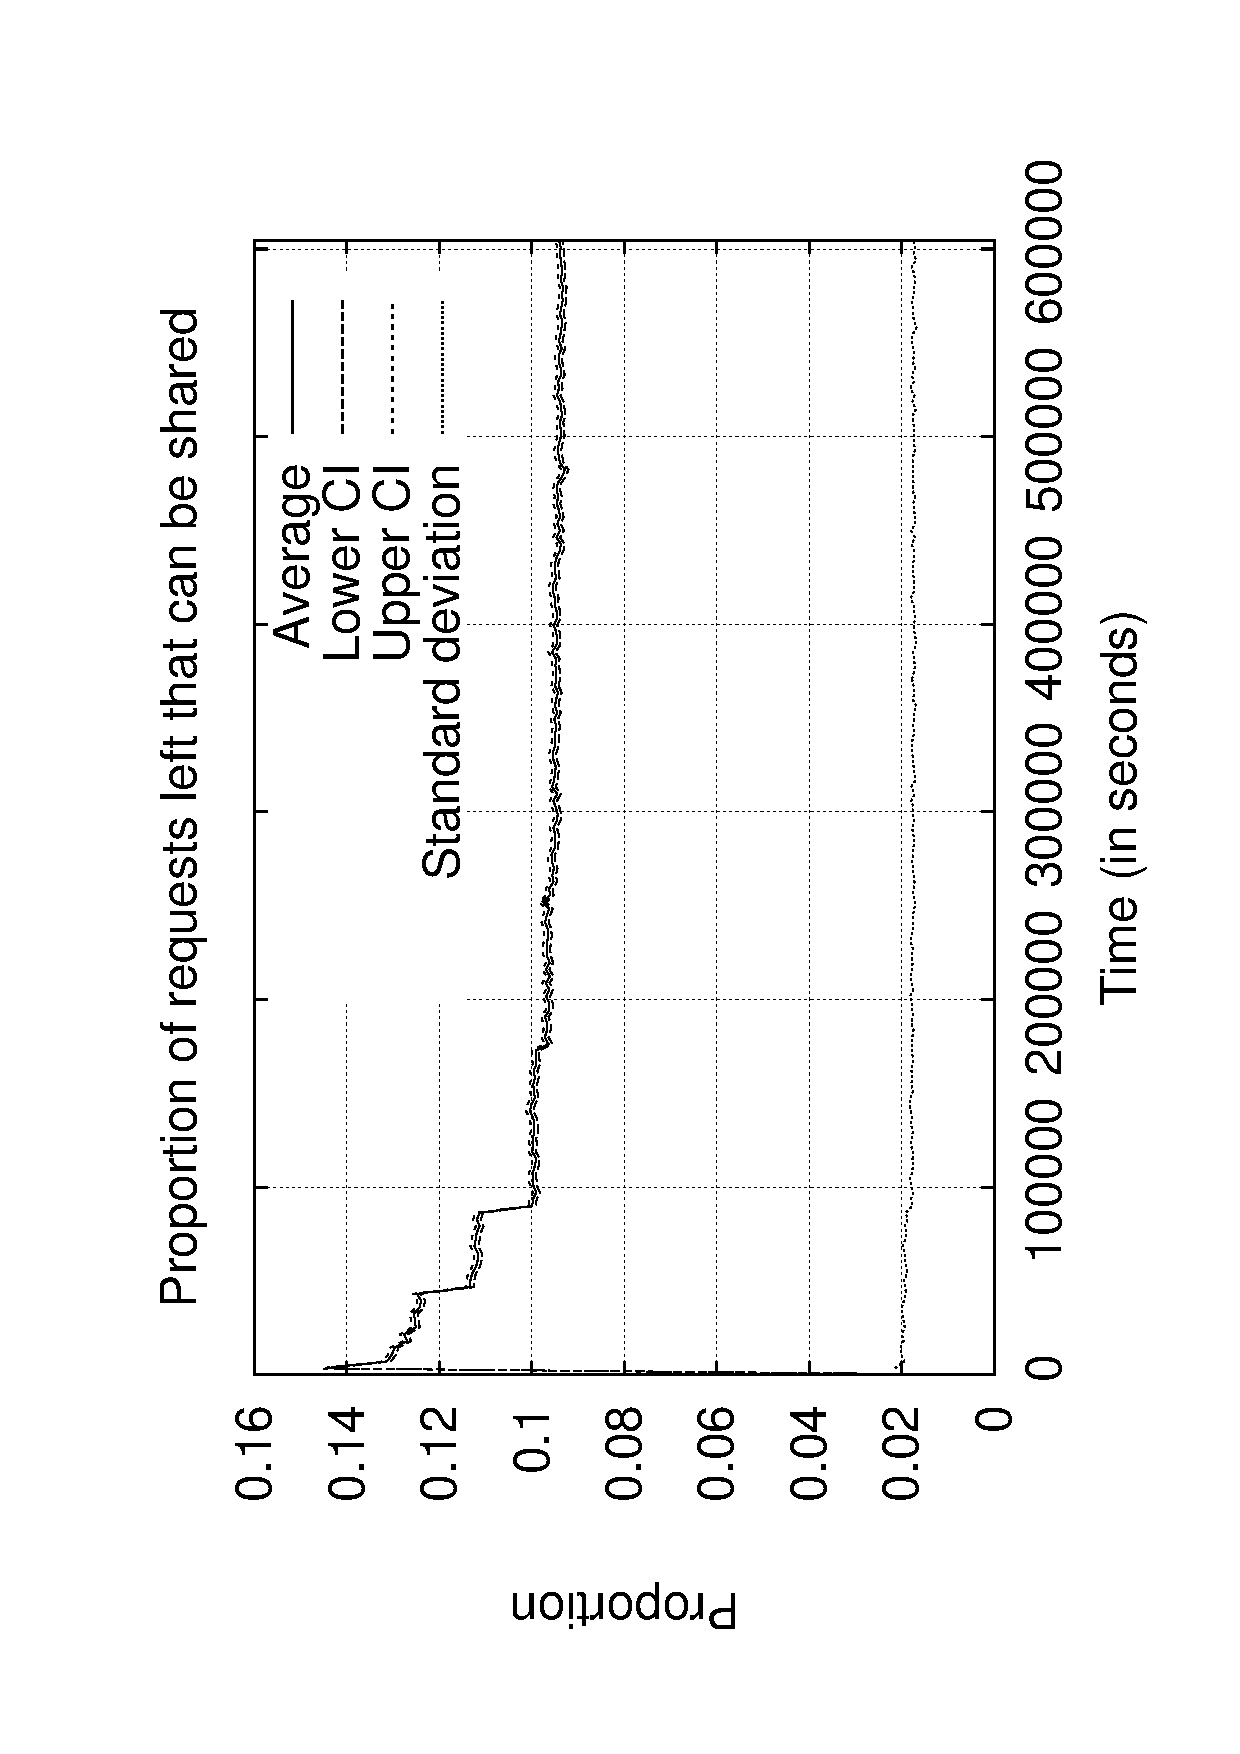
\includegraphics[width=.95\linewidth]{savings_Sum_of_requests_over_time}
%	\caption{multiplied}
%	\label{fig:sim_saver}
%\end{figure}
%
%\begin{figure}
%	\centering
%	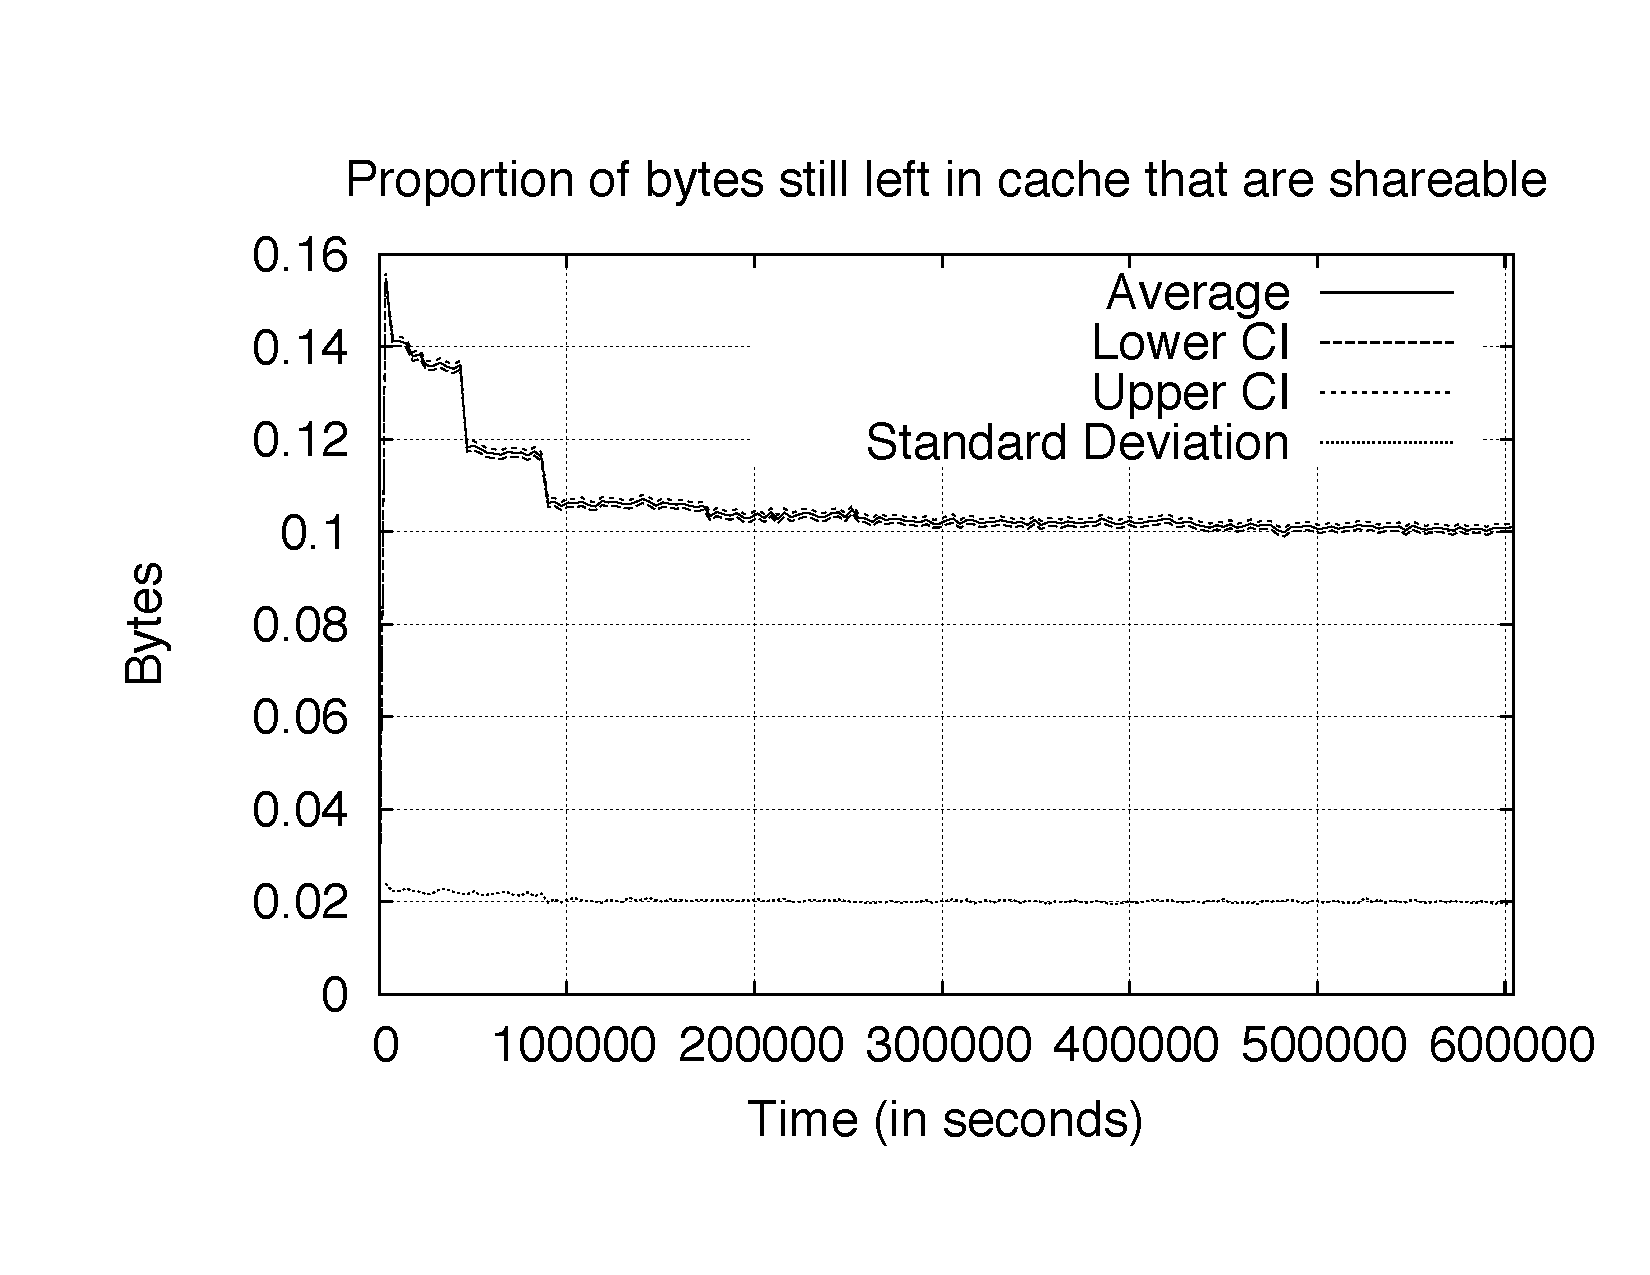
\includegraphics[width=.95\linewidth]{savings_Sum_of_bytes_over_time}
%	\caption{multiplied}
%	\label{fig:sim_saveb}
%\end{figure}

%We additionally evaluate the impact of the Zipf distribution's $\alpha$ parameter. 
%While we omit detailed results due to space constraints, we find that all levels of $0.65 \le \alpha \le 1.05$ exhibit the same underlying trends, with slight and non-linear differences between levels.
To evaluate the impact of different web page popularity distributions, we present an evaluation of different $\alpha$ for the Zipf distribution in Figure~\ref{fig:sim3}, each with 500 simulation repetitions for $0.65 \le \alpha \le 1.05$.
%\begin{figure*}[]
%	\centering
%	\subfloat[Requests]{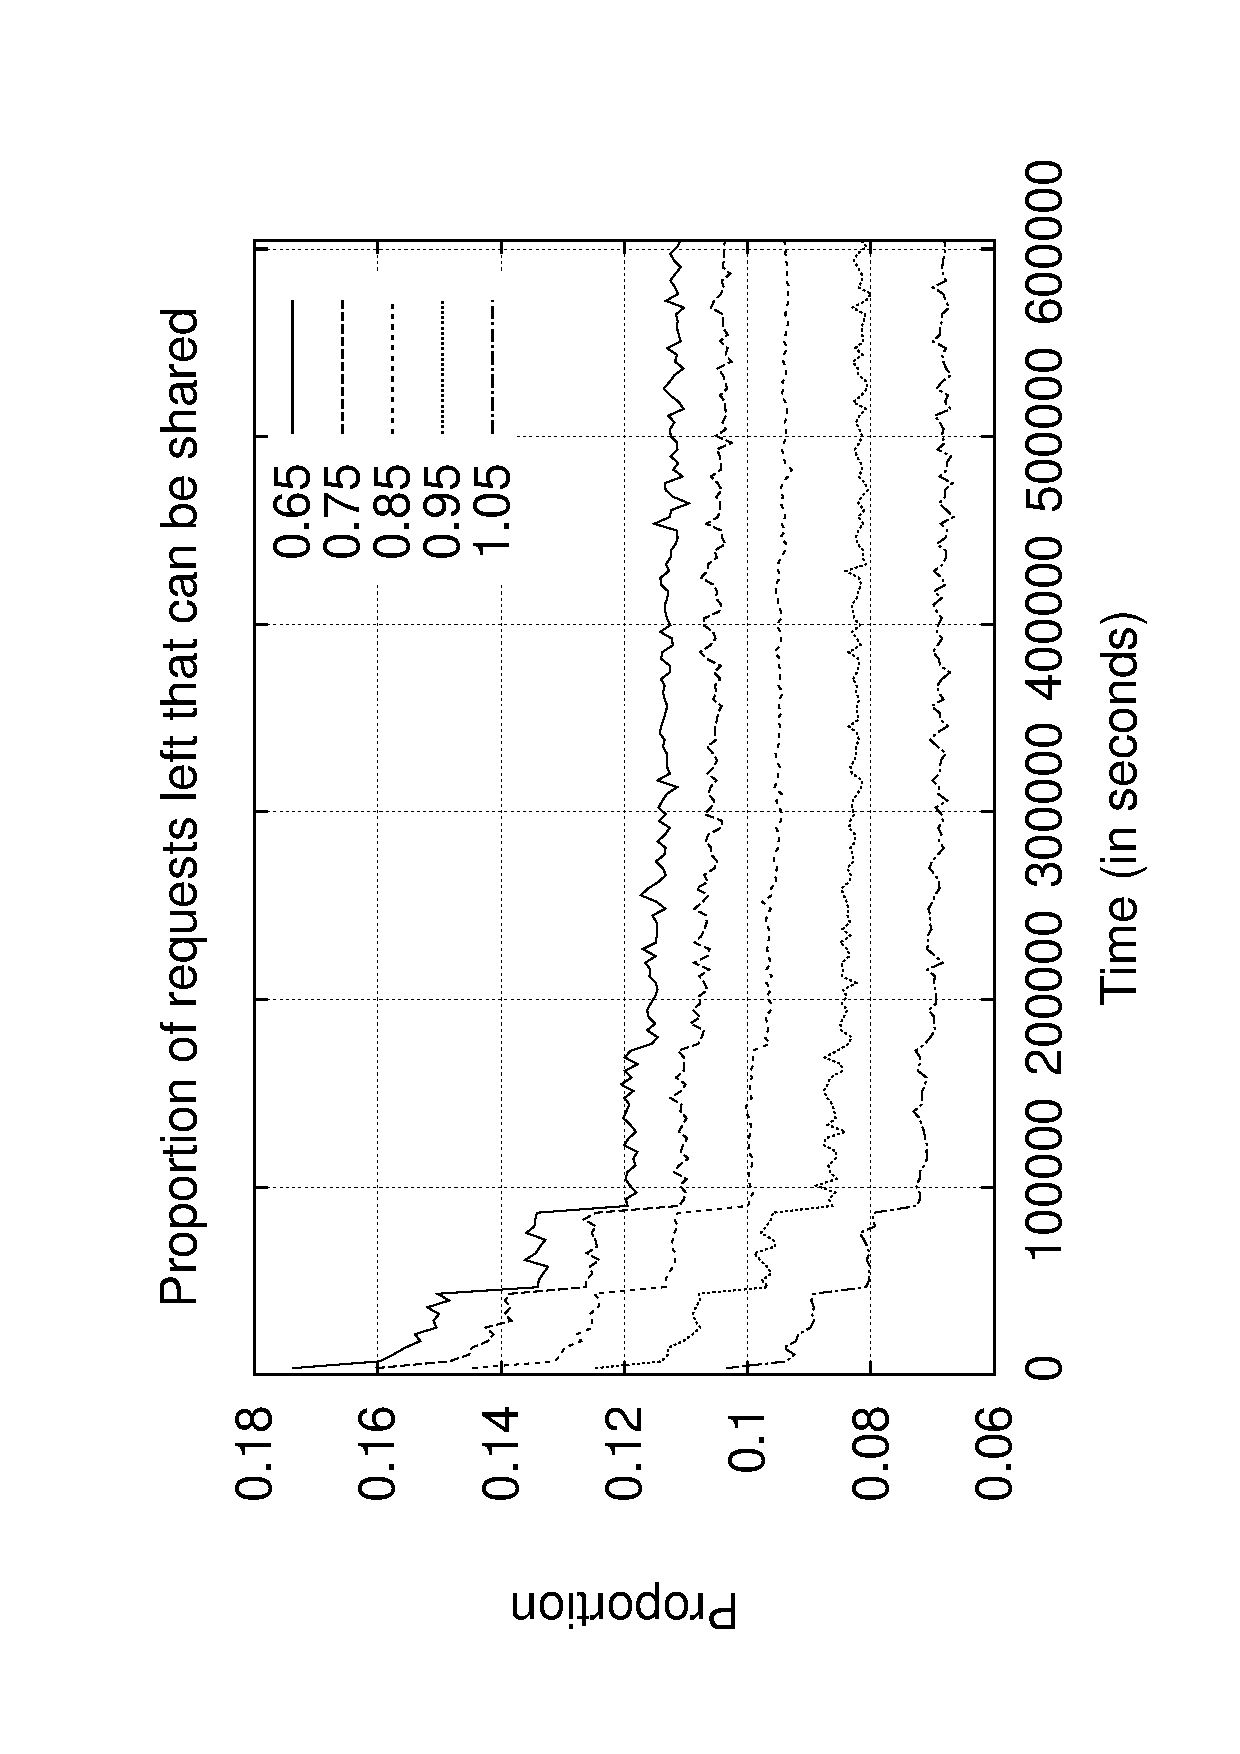
\includegraphics[width=.4\linewidth]{Sum_of_requests_over_time_overview}
%	\label{fig:simr_zipf_reqs}}
%	\hfil
%	\subfloat[Bytes]{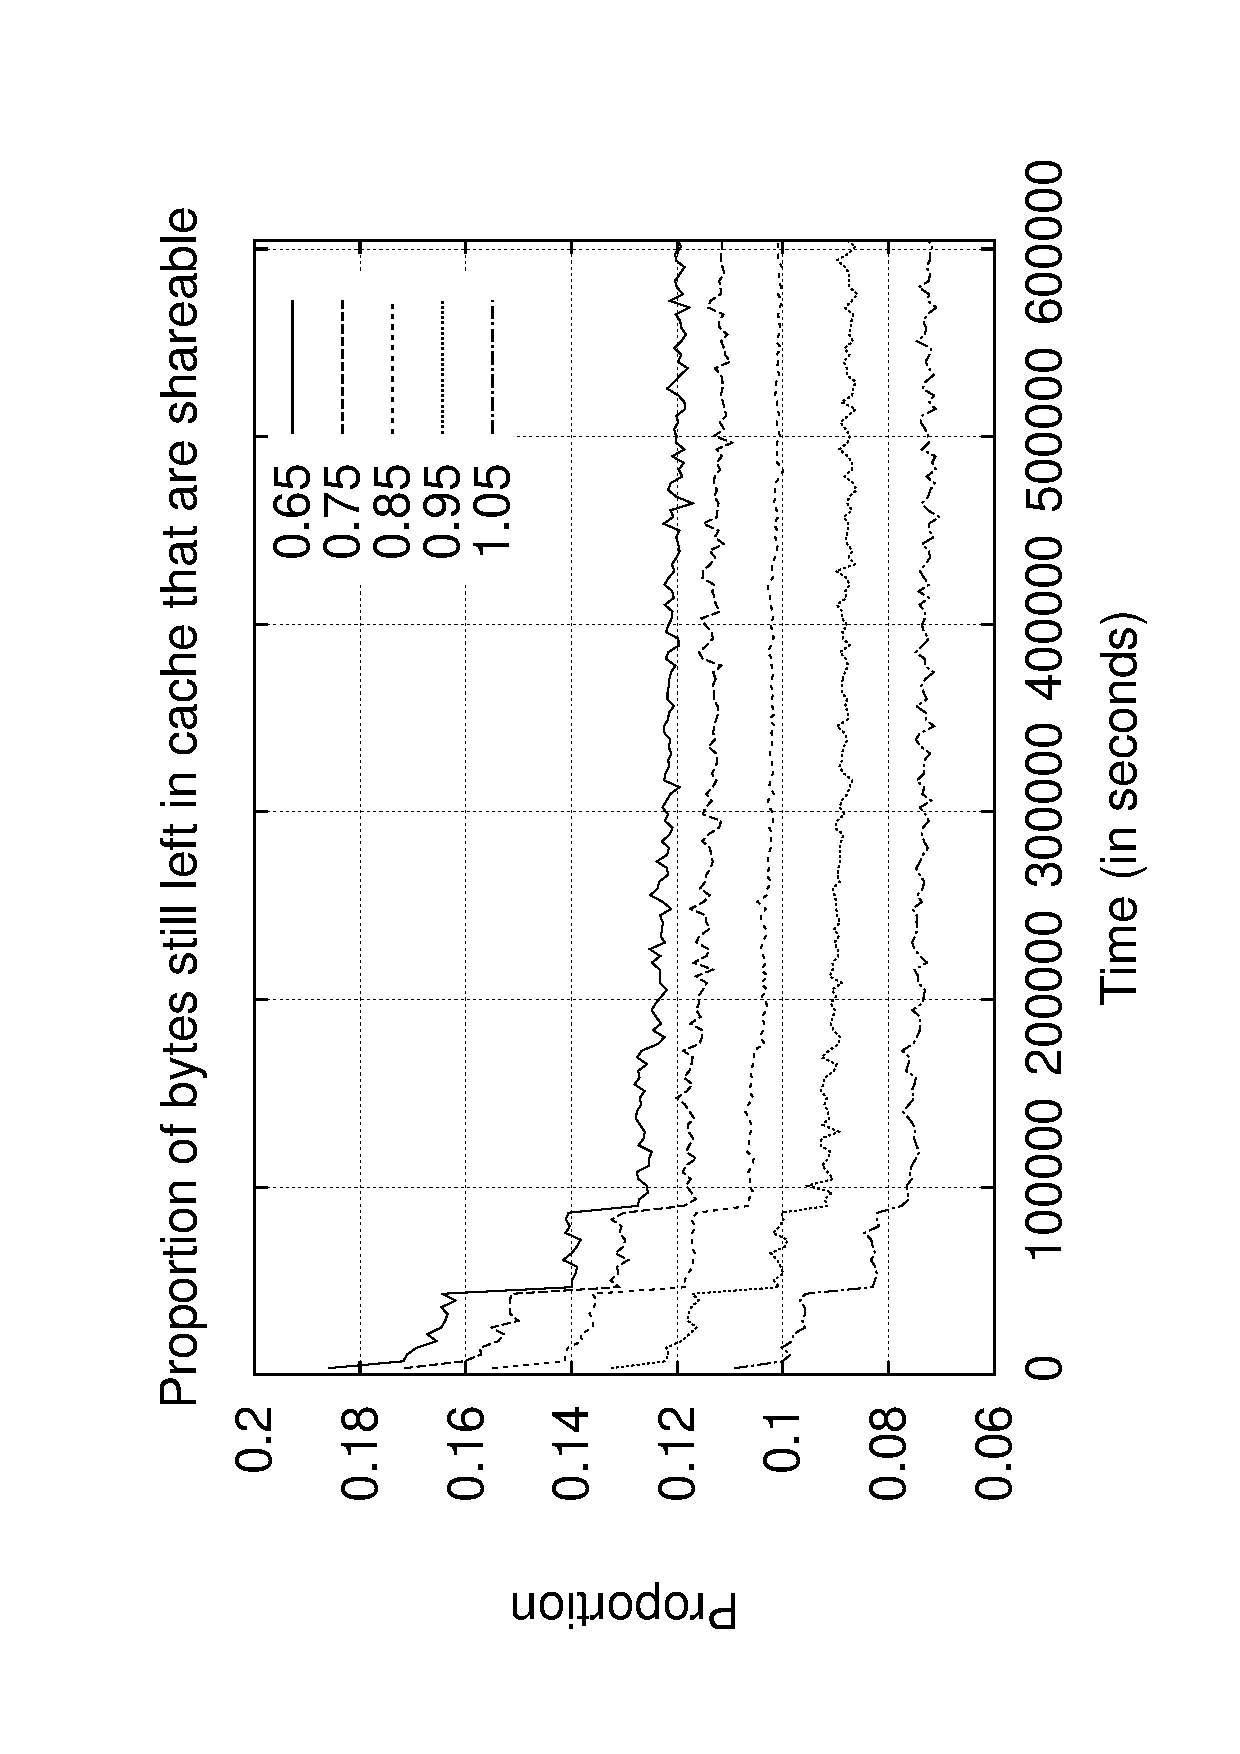
\includegraphics[width=.4\linewidth]{Sum_of_bytes_over_time_overview}
%	\label{fig:simr_zipf_byte}}
%	\caption{Simulation results for the attained savings for the number of responses and bytes for different levels of $\alpha$ for the underlying Zipf distribution.}
%	\label{fig:sim3}
%\end{figure*}
We limit our comparison to bytes due to space constraints, noting that results obtained for objects are similar.
\begin{figure}[]
	\centering
	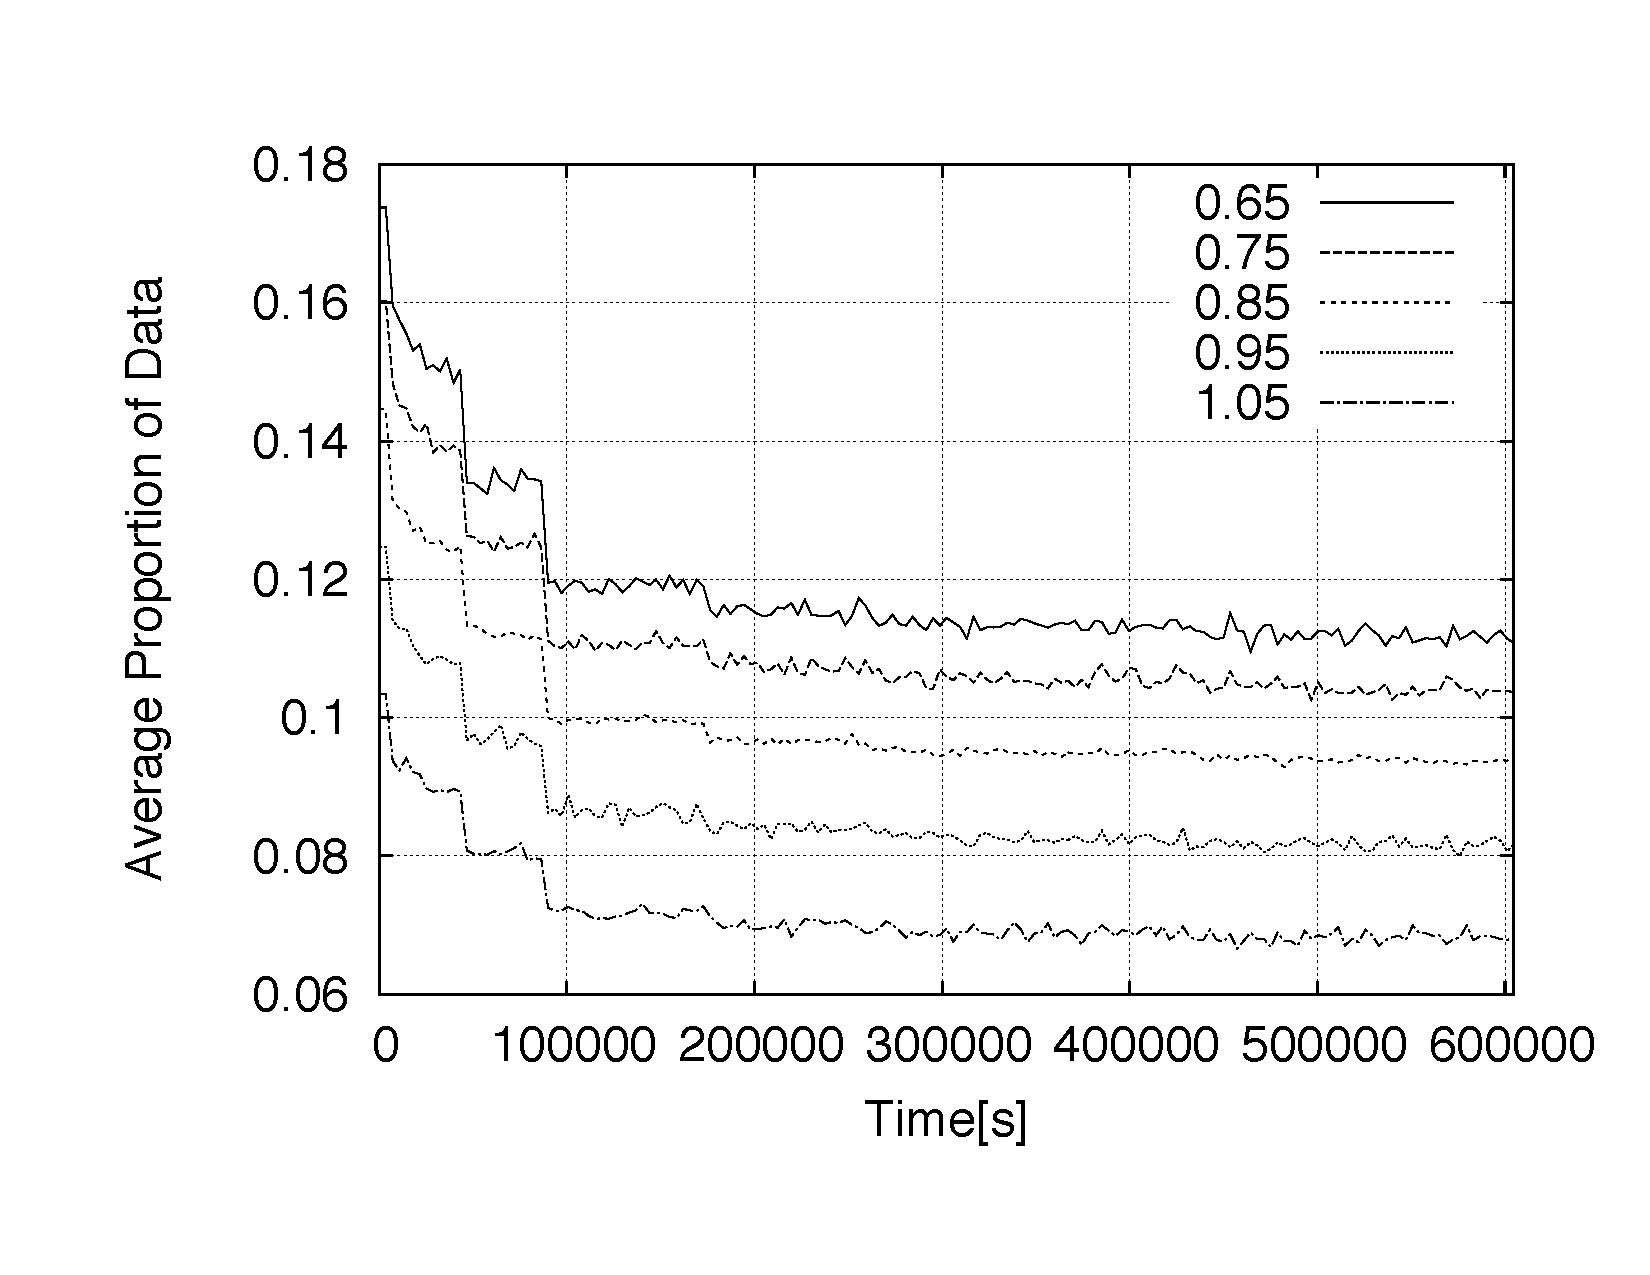
\includegraphics[width=.5\textwidth]{Fig8}
	\caption{Average proportions of data in mobile cache for different Zipf distribution parameters $\alpha$.}
	\label{fig:sim3}
\end{figure}
We observe that all levels of $\alpha$ exhibit the same underlying trends, with slight and non-linear differences between levels.
We conclude that the distribution of web page popularity and the composition thereof has an overall impact on the long-term level of savings that can be attained.
%\begin{figure}
%	\centering
%	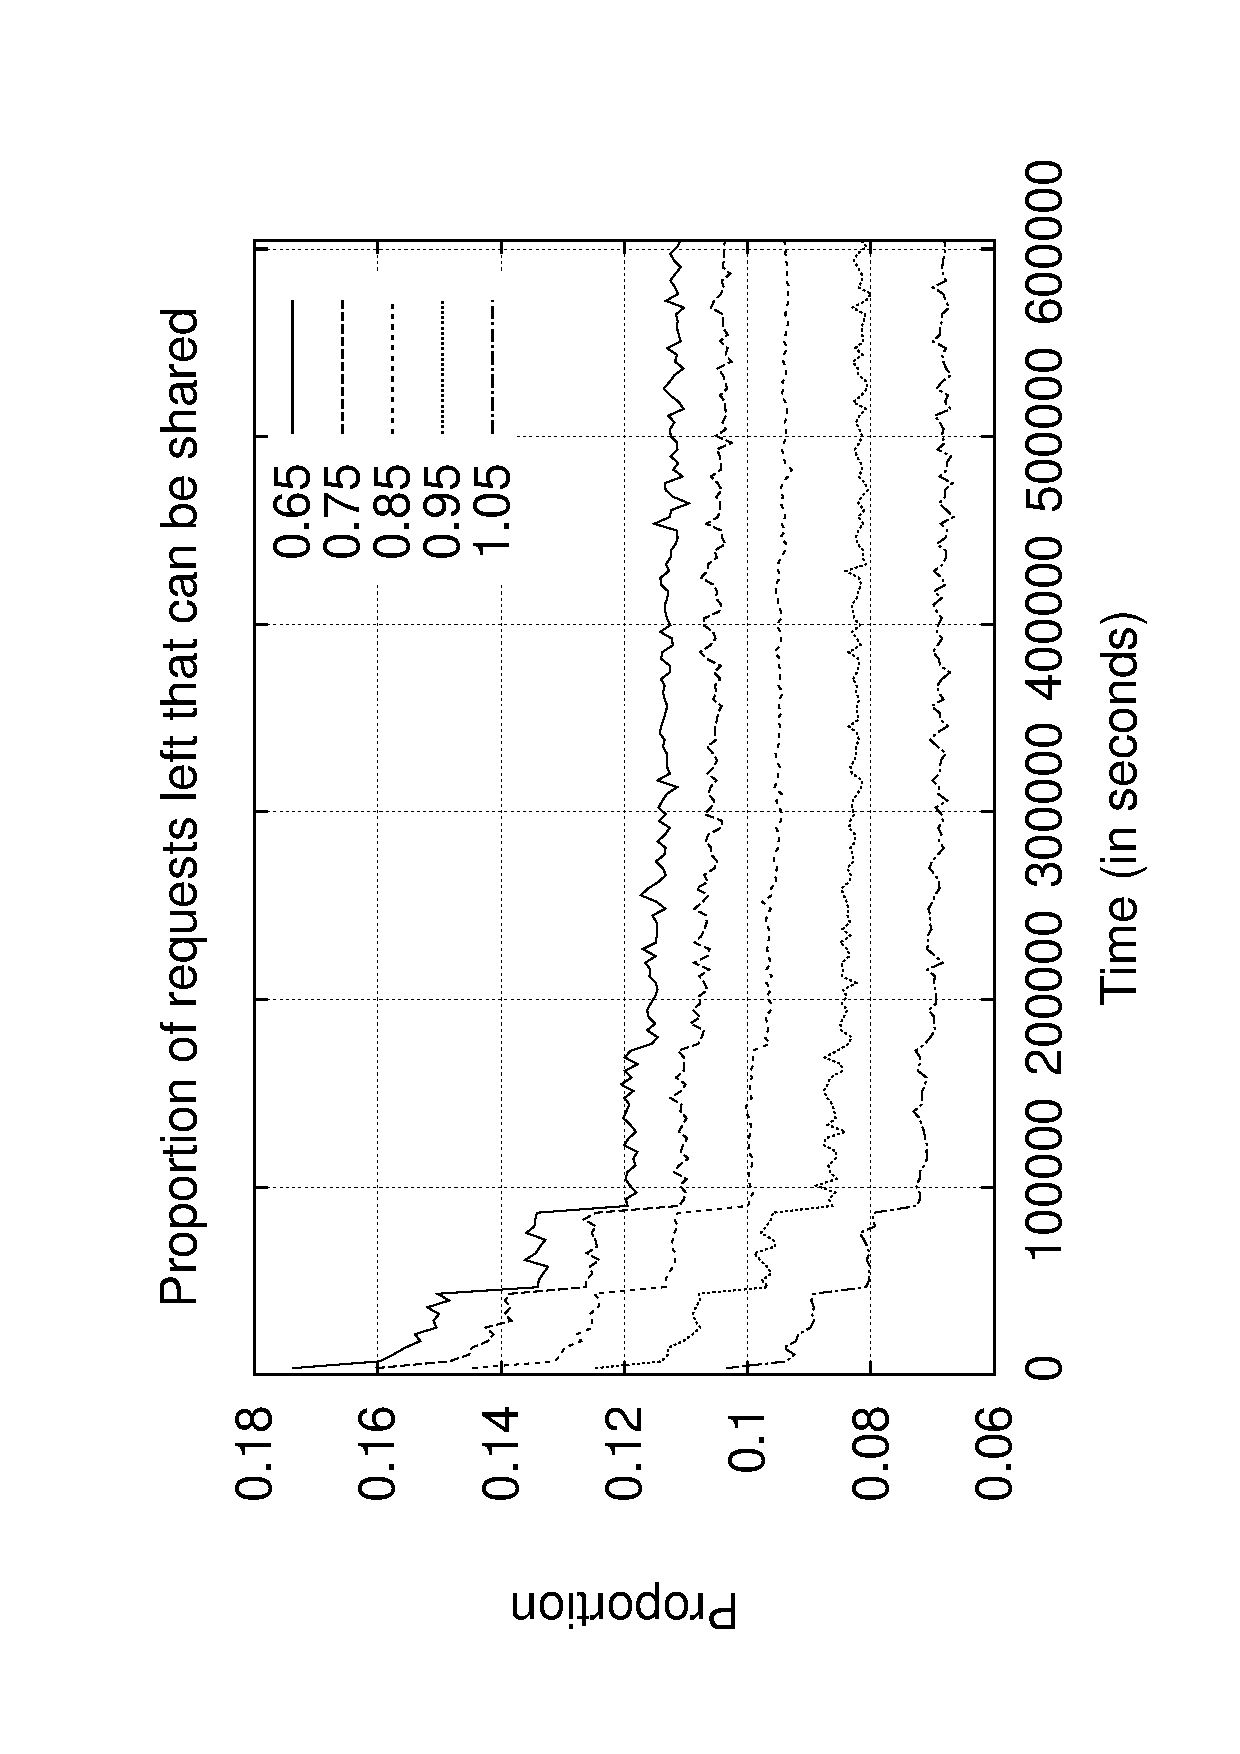
\includegraphics[width=.95\linewidth]{Sum_of_requests_over_time_overview}
%	\caption{multiplied}
%	\label{fig:sim_saveb}
%\end{figure}

\subsection{Discussion}
Overall, we find a significant reduction in the required downloads for mobile clients that can be directly attributed to lower energy consumption levels and potential download latencies (and even costs for the mobile user through saved data transmissions).
Furthermore, this approach does not require sophisticated live evaluations, but only relies on cache forwarding to the mobile device.
\uline{These savings are additionally passed on to cellular network providers, assuming that users empty their devices in their co--located home networks. 
In this case, the exchange of data can be performed either directly in a device--to--device manner with cellular network operator control or independently between devices locally networked, e.g., through commonly employed integrated wireless access points.}

\uline{Comparing our simulation results to other current approaches, we find that our scheme lies well within commonly attained savings reported.
If sending web objects as bundles to users within a cell coverage area, for example, it was found in~\cite{Finamore:2013dn} that significant savings can be attained. 
Mechanisms that work as mobile devices are in use, however, can potentially have negative impacts due to an increase in the resulting network traffic, as reported in~\cite{Marquez:2008wf} to potentially reach upwards of 25 \%, effectively reducing battery length of service, predominantly caused by low cache hit rates of the downloaded content~\cite{Wang:2012ks}. Similarly, these schemes might have an increased network burden for cellular service providers.
Our proposed scheme does not suffer from this particular drawback, as it works while devices are commonly charged over night utilizing a user's commonly unmetered home network.}

\uline{Similar to our approach, in~\cite{Qian:2014dw}, the authors evaluate web landing pages and their characteristics as well as caching potentials. Their findings indicate that the difference between a warm and cold cache is approximately 20 \% on average, which is similar to our findings. 
Specifically, as our approach pre--populates the mobile device's browser cache, it can be regarded as an example implementation to ``warm up'' the mobile cache.}

\uline{With a majority of mobile users employing additional means of accessing content (such as through dedicated mobile applications for a web site as well as subscription--based services), these alternative means are becoming optimization subjects as well.
For mobile applications, a device--level intercepting caching system for Android mobile applications shows significant traffic reduction, see~\cite{Zhang:2013}.
The authors of~\cite{Wang:2014di} found that with a cloud assisted pre--fetching system and cognitive pushing, anywhere from 43 to 73 \% of traffic load can be reduced for feed--based subscriptions.
}


\section{Conclusion}
\label{s:conc}
We exemplarily evaluated the content of modern web pages and the identical objects that can be found when requesting the same web page from different devices with different display modalities, such as desktop and smartphone.
Assuming mobile users visit the same pages on their mobile device that they visit on their desktop computer as well, we simulated the access of landing web pages and evaluated the potential for \uline{web object forwarding to generate a warm cache on the mobile device}.
Our basic approach is able to save upward of 7.5 \% of mobile requests or bytes, even for very distant time horizons.
In most typical daily time ranges, our approach can yield almost linearly decreasing savings starting at about 14 \%, without requiring any sophisticated prediction mechanisms, but only a direct cache transfer.
\uline{Since this approach can be implemented directly between devices or using a user's home network, it is also suitable to be employed in device--to--device (D2D) scenarios aiding cellular network providers to offload traffic}.
We note that similarly, exchanges between mobile and fixed devices belonging to a user are possible, including keeping a cloud-based reference of pages that a user visits (similar to Google Chrome's synchronization features). %, which is the subject of our ongoing work. 
%We similarly note that incorporation of predictive caching and user context can with little overhead increase the outlined savings, which represents another current research venue.

\IEEEtriggeratref{7}
\bibliographystyle{IEEEtran}
\bibliography{content}


\end{document}
